\chapter{Análise dos resultados}\label{ch:resultados}
A ideia deste capítulo é trazer uma visão geral sobre todas as funcionalidades desenvolvidas, o fluxo de navegação entre as \textit{features} e como o \ac{app} ficou em sua última versão.

\section{Apresentação do Enzitech}
Após concluído todos os requisitos funcionais, a versão final do Enzitech lida com dois tipos de usuário, Comum ou Administrador. O primeiro deles é referente ao perfil de todos os usuários, pessoas que utilizarão o sistema para criar e calcular seus experimentos. Já o segundo é destinado ao administrador geral de todo o sistema, normalmente uma única pessoa que ficará encarregada de gerir o Enzitech disponibilizando os dados corretamente. 

A diferença entre os dois perfis está na possibilidade de criação de enzimas, funcionalidade restrita ao Administrador, devido a necessidade de ajuste também no \textit{back-end}, ou seja, o Administrador fica responsável por gerir (criar e excluir) enzimas e solicitar a inclusão de novos cálculos para outros tipos, outro detalhe importante é que as enzimas criadas pelo Administrador ficam disponíveis para todos os usuários do sistema, as demais funcionalidades ficam disponíveis para ambos os tipos de usuário. 

Sendo assim, para ter acesso ao sistema, o usuário terá que inserir seus dados de acesso, e-mail e senha, na tela de login (\figref{fig:fluxo_login}). A autenticação é fundamental para que o usuário tenha acesso às funcionalidades do \ac{app}, o login satisfaz o caso de uso UC02.


\begin{figure}[H]
\centering

\includegraphics[width=.3\textwidth]{images/enzitech/splash.png}
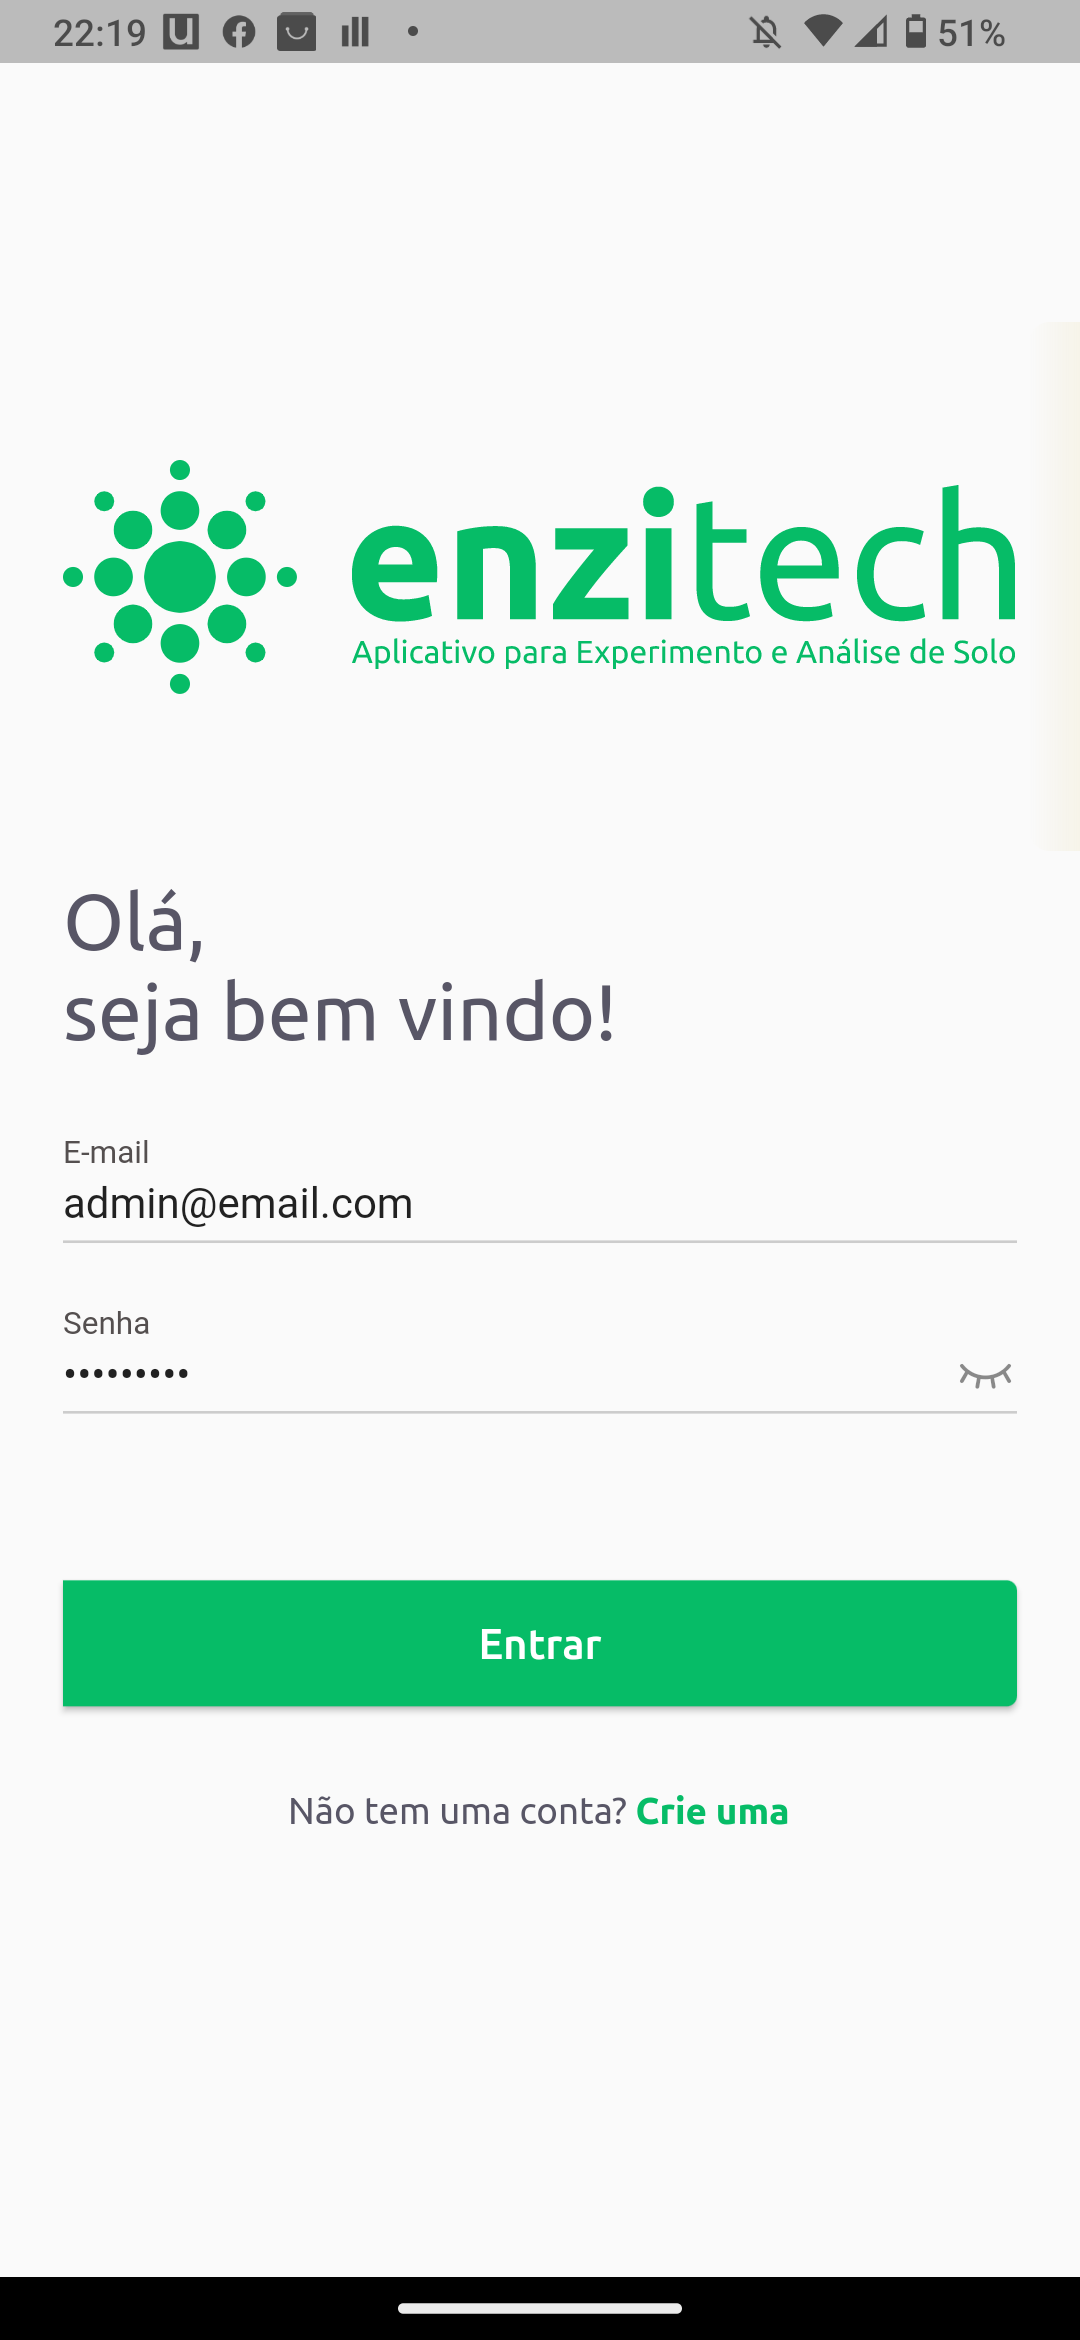
\includegraphics[width=.3\textwidth]{images/enzitech/login.png}
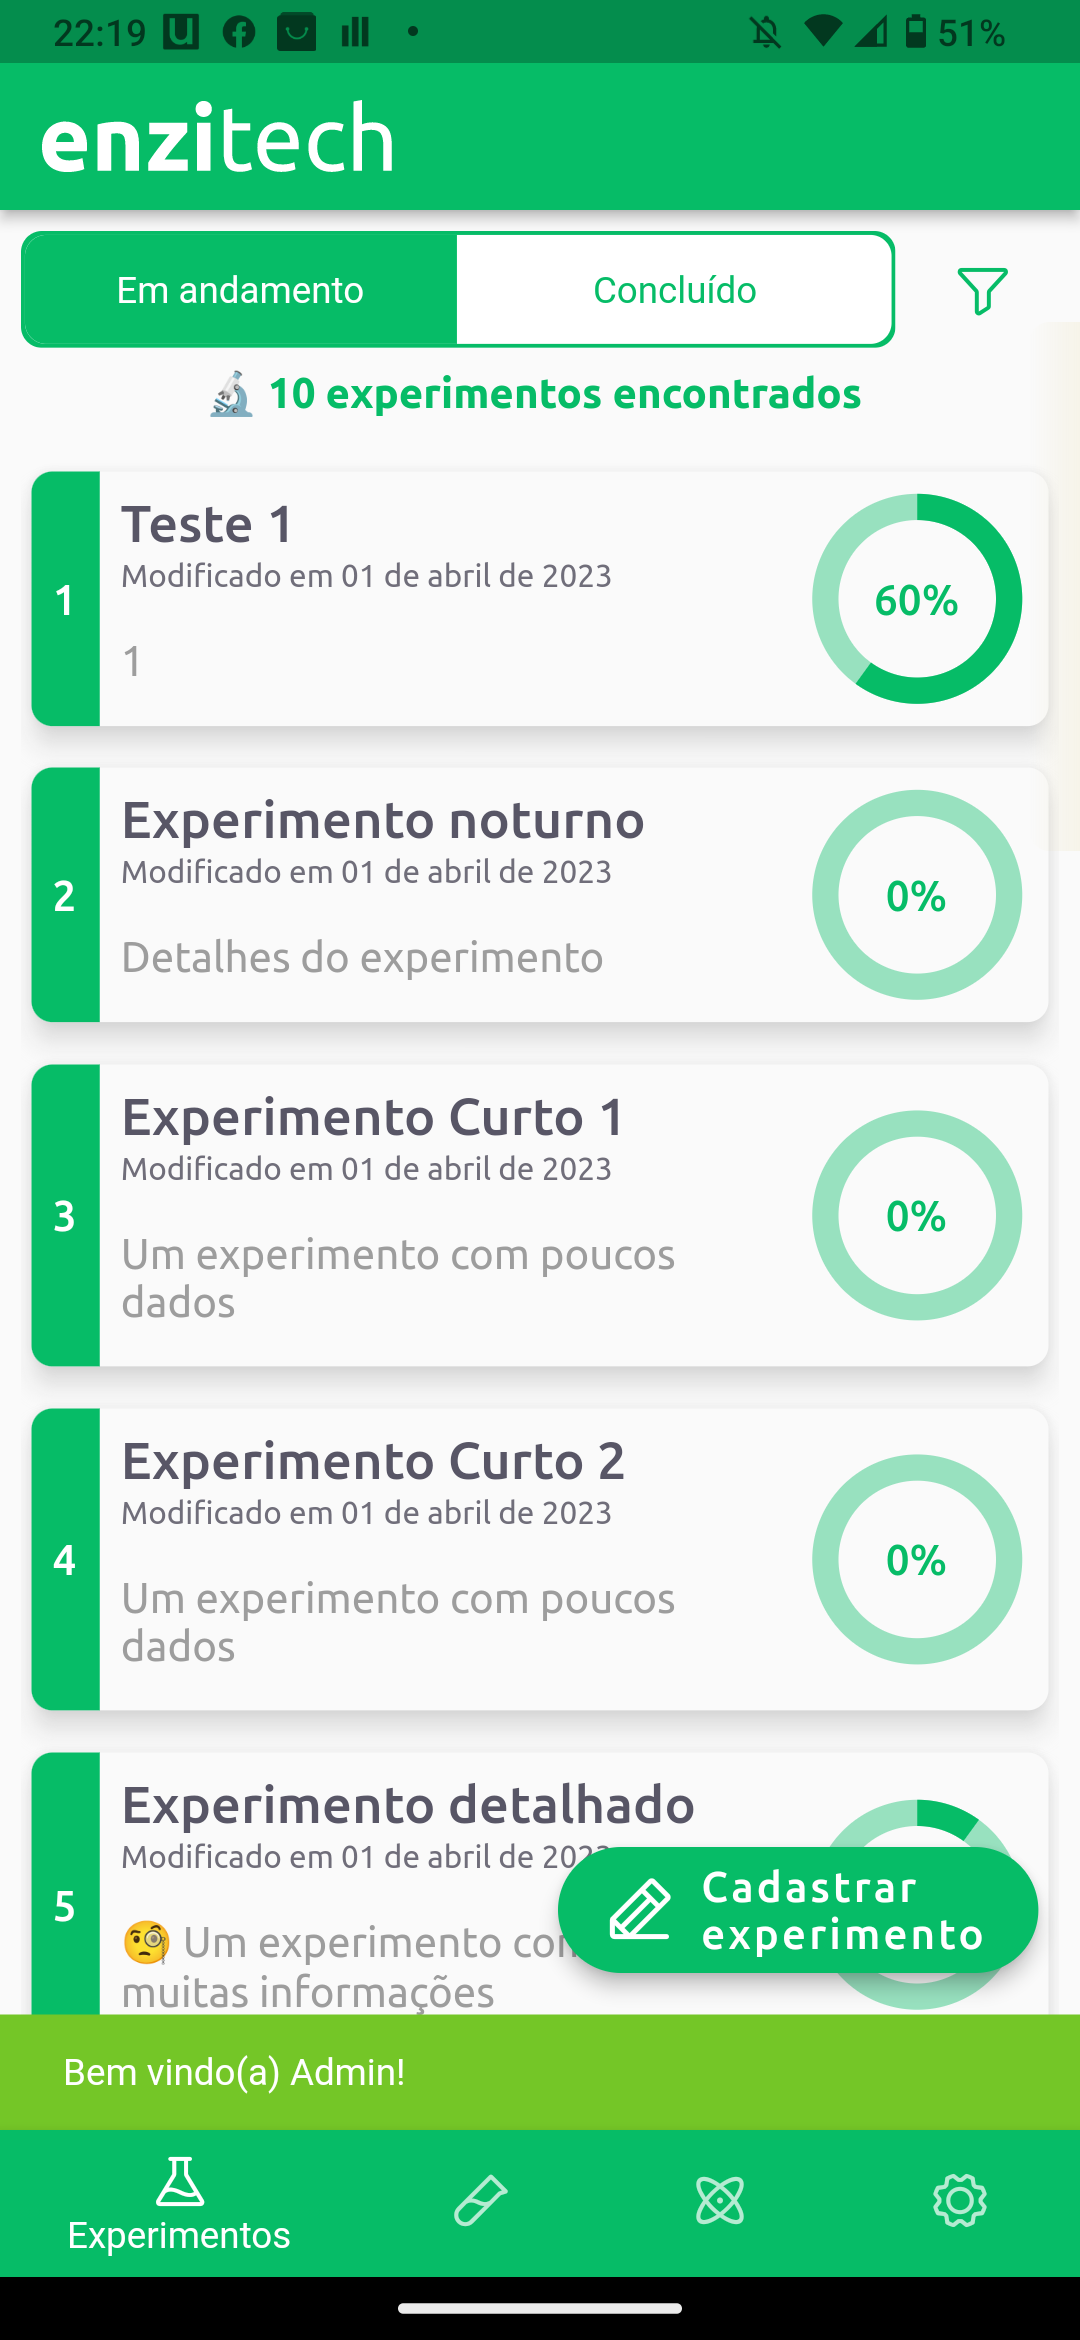
\includegraphics[width=.3\textwidth]{images/enzitech/home.png}
\caption{Fluxo de login do Administrador previamente cadastrado}
\acsfont{Fonte: Aplicativo Enzitech desenvolvido pelo autor}
\label{fig:fluxo_login}
\end{figure}

Na \figref{fig:fluxo_login} é possível ver o fluxo inicial do \ac{app}, ao abrí-lo, é feita uma verificação na \textit{splashscreen} (primeira imagem da sequência) para determinar se existe usuário logado ou não, caso negativo, o \ac{app} redireciona para a tela de login, onde é possível criar uma conta (caso de uso UC01), recuperar senha (caso de uso UC03) ou logar com suas credencias, após o login, ou, caso o usuário já estivesse logado, o app redireciona para a \textit{homepage}, onde estão todas as funcionalidades disponíveis, a primeira delas é a listagem de experimentos (caso de uso UC07), nesta tela é possível além da listagem, filtrar, excluir ou criar, como será mostrado em breve.

\begin{figure}[H]
\centering
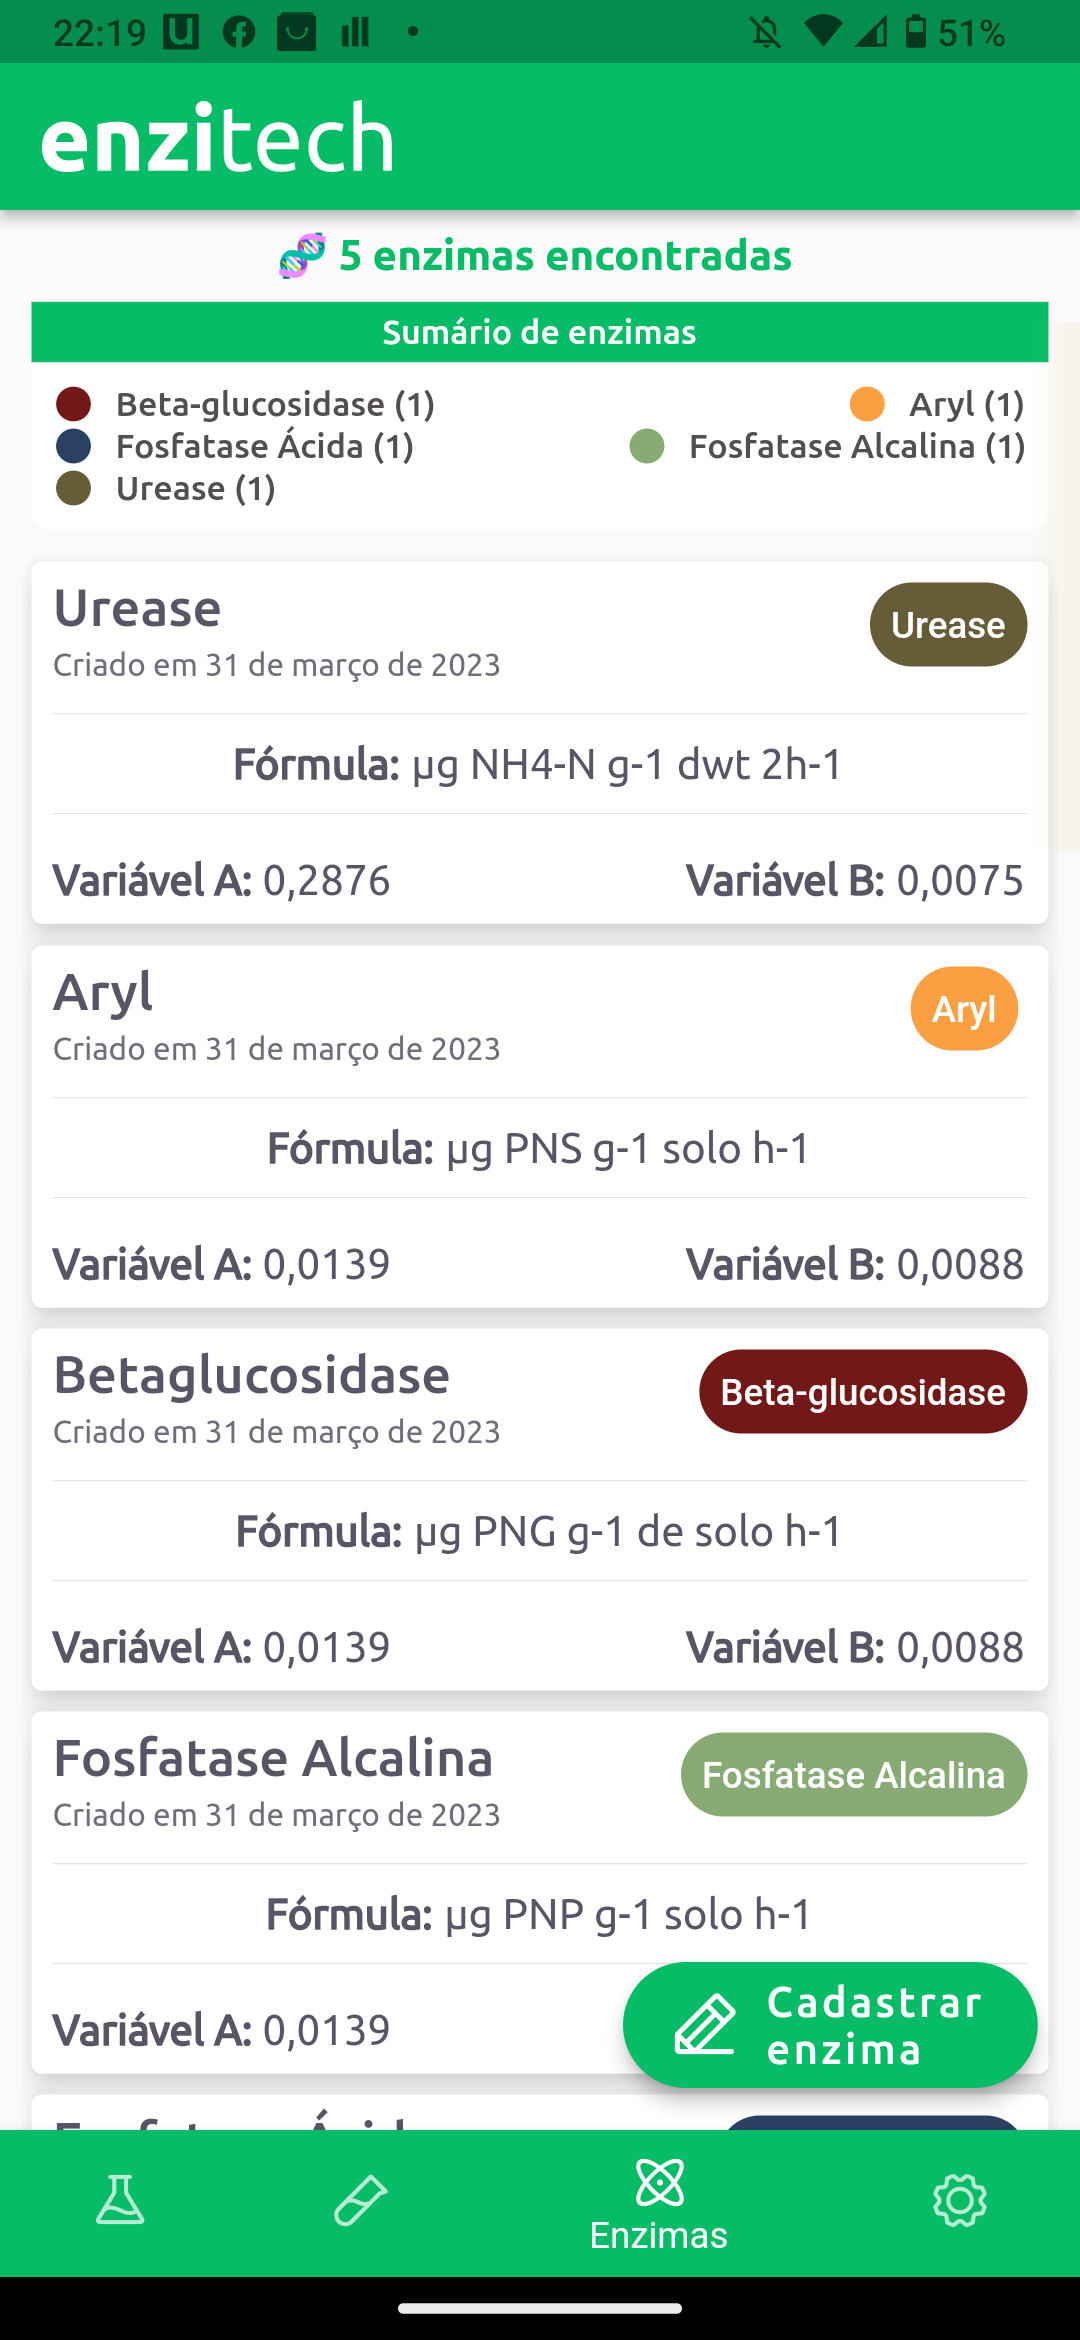
\includegraphics[width=.4\textwidth]{images/enzitech/enzimas.png}\hfill
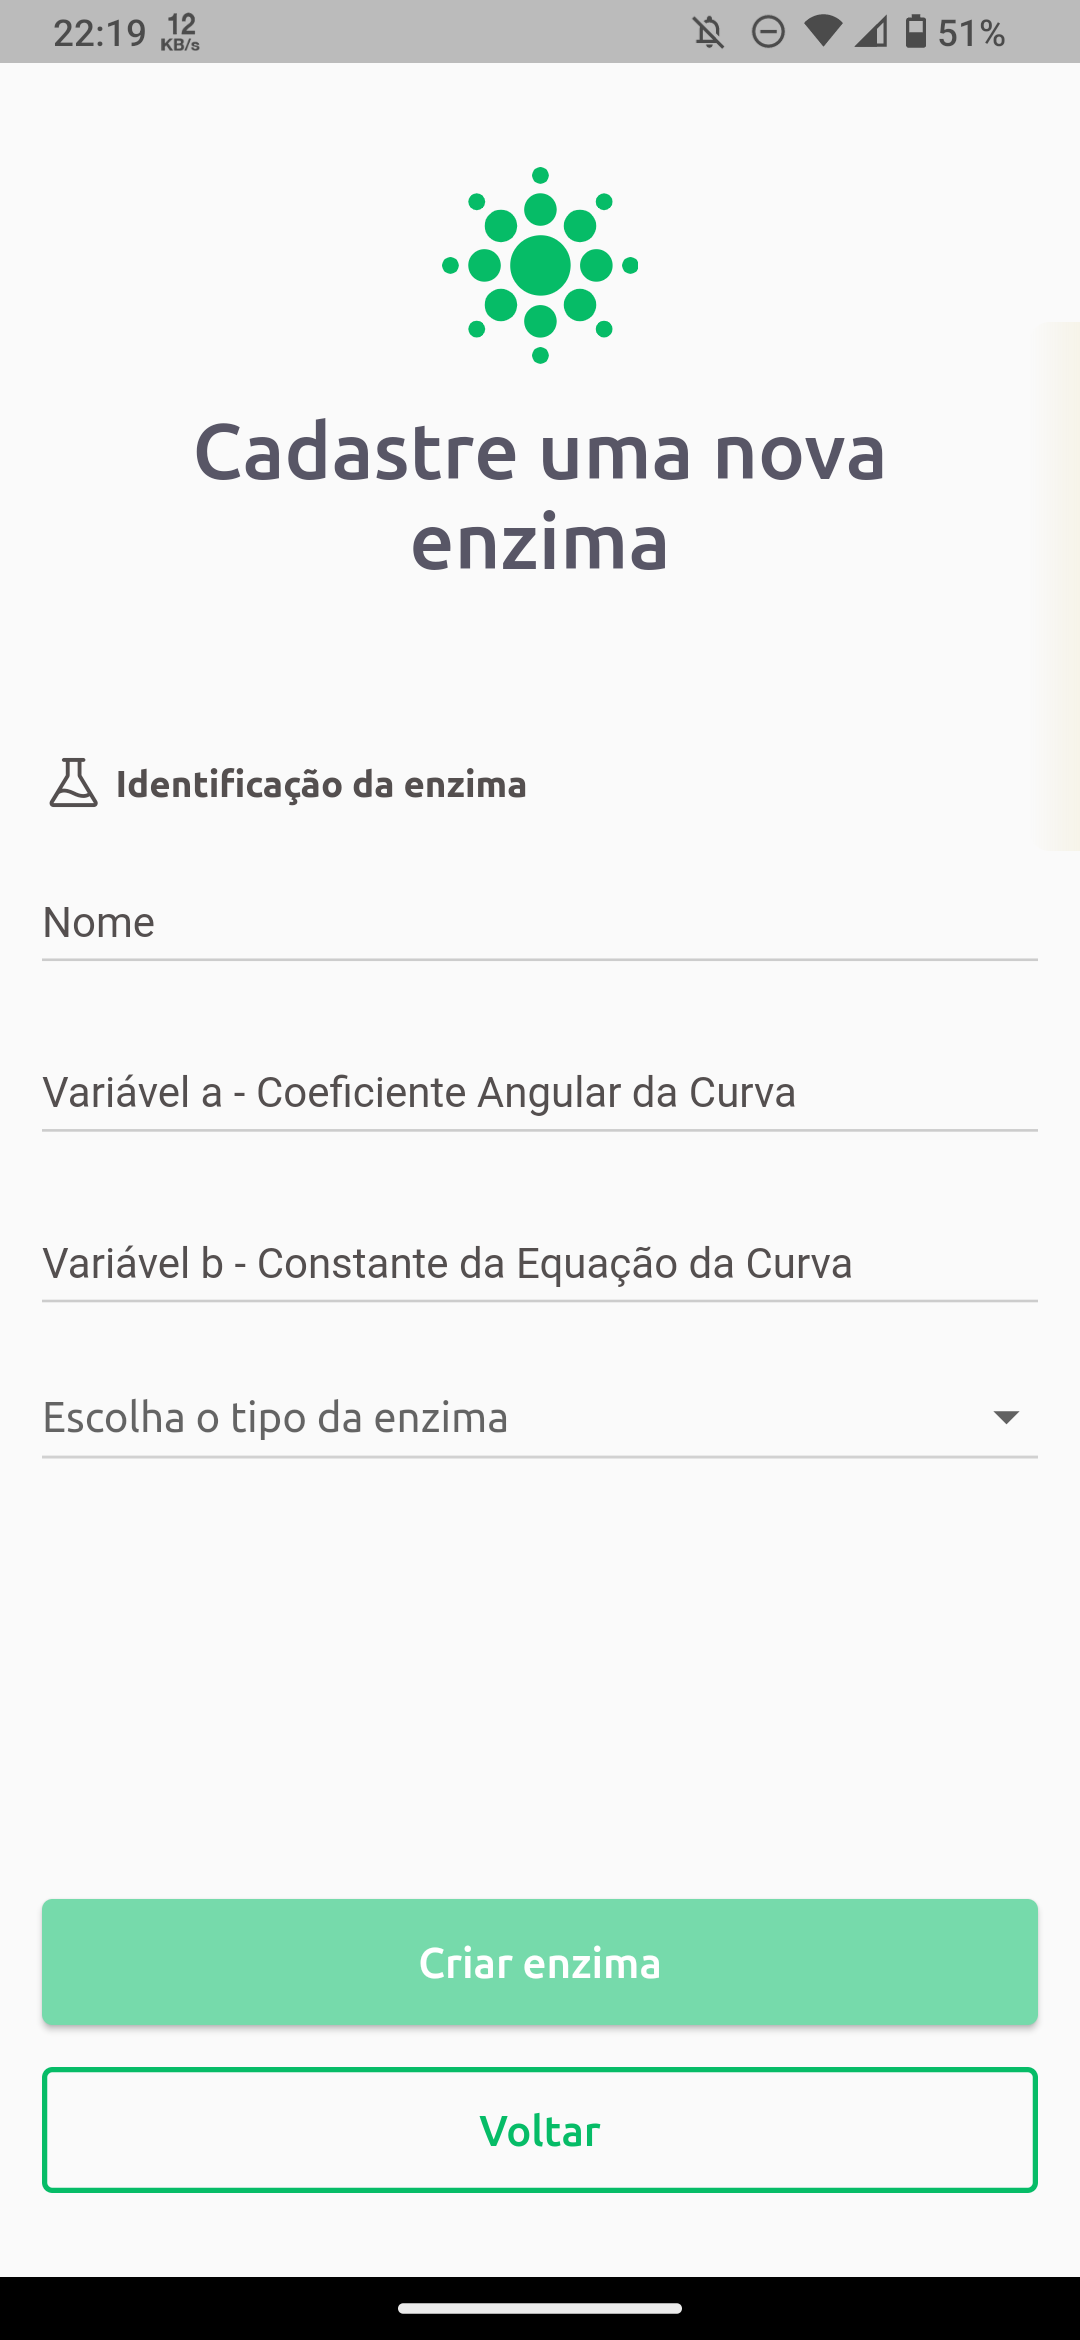
\includegraphics[width=.4\textwidth]{images/enzitech/cria_enzima.png}\hfill
\caption{Fluxo de listagem, exclusão e criação de enzimas}
\acsfont{Fonte: Aplicativo Enzitech desenvolvido pelo autor}
\label{fig:fluxo_enzima}
\end{figure}

Na \figref{fig:fluxo_enzima} estão as funcionalidades de listagem, exclusão e criação de enzimas, esta última restrita ao administrador, satisfazendo os casos de uso UC05 e UC06. Criar uma enzima no sistema é fundamental para a criação de um experimento.

Abaixo, na \figref{fig:fluxo_tratamento}, está o fluxo de listagem, criação e exclusão dos tratamentos (caso de uso UC04), a criação de um tratamento também é fundamental para a criação de um experimento.

\begin{figure}[H]
\centering
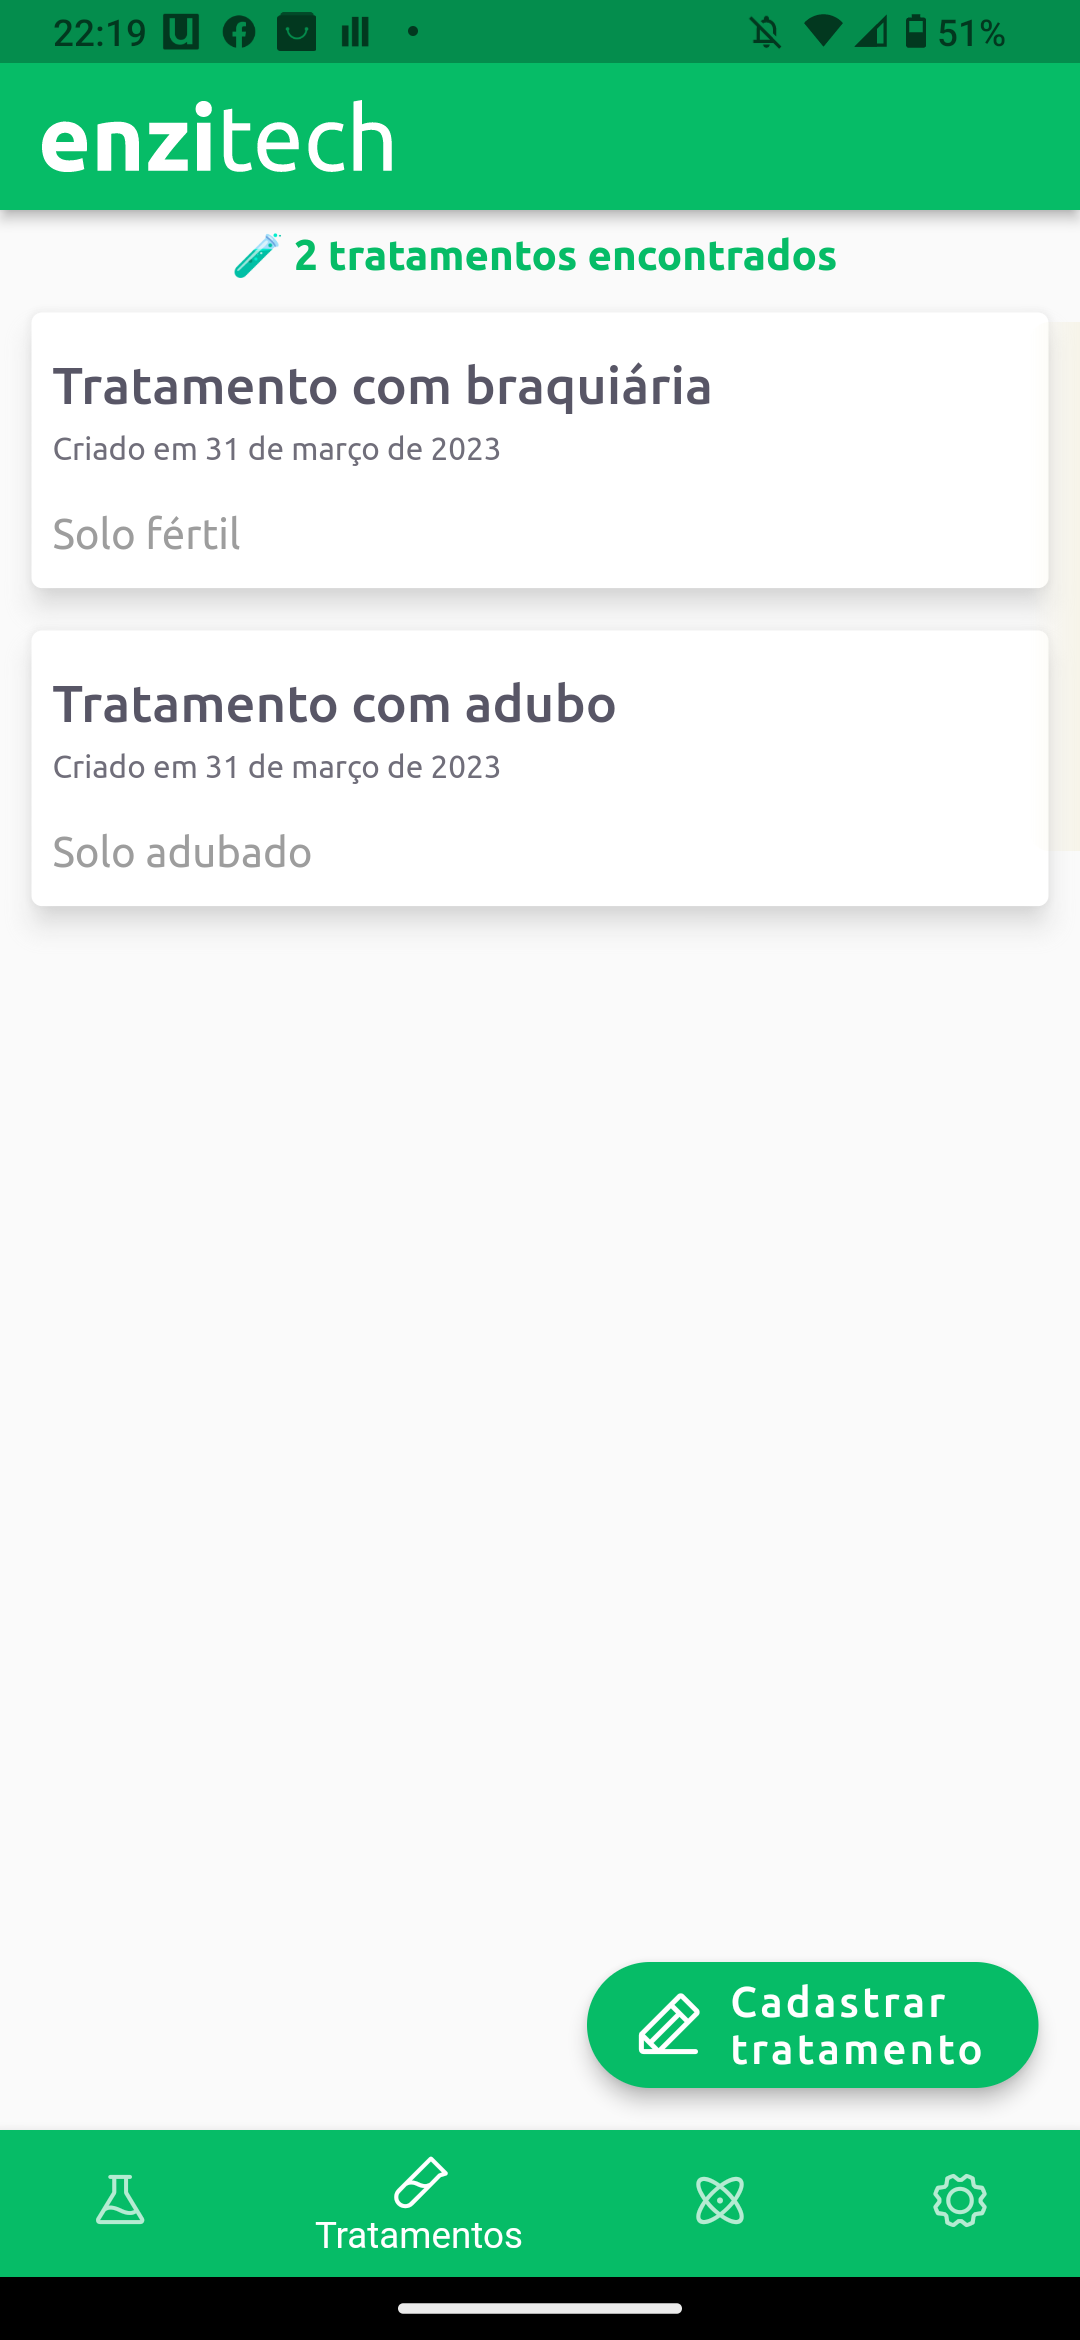
\includegraphics[width=.4\textwidth]{images/enzitech/tratamentos.png}\hfill
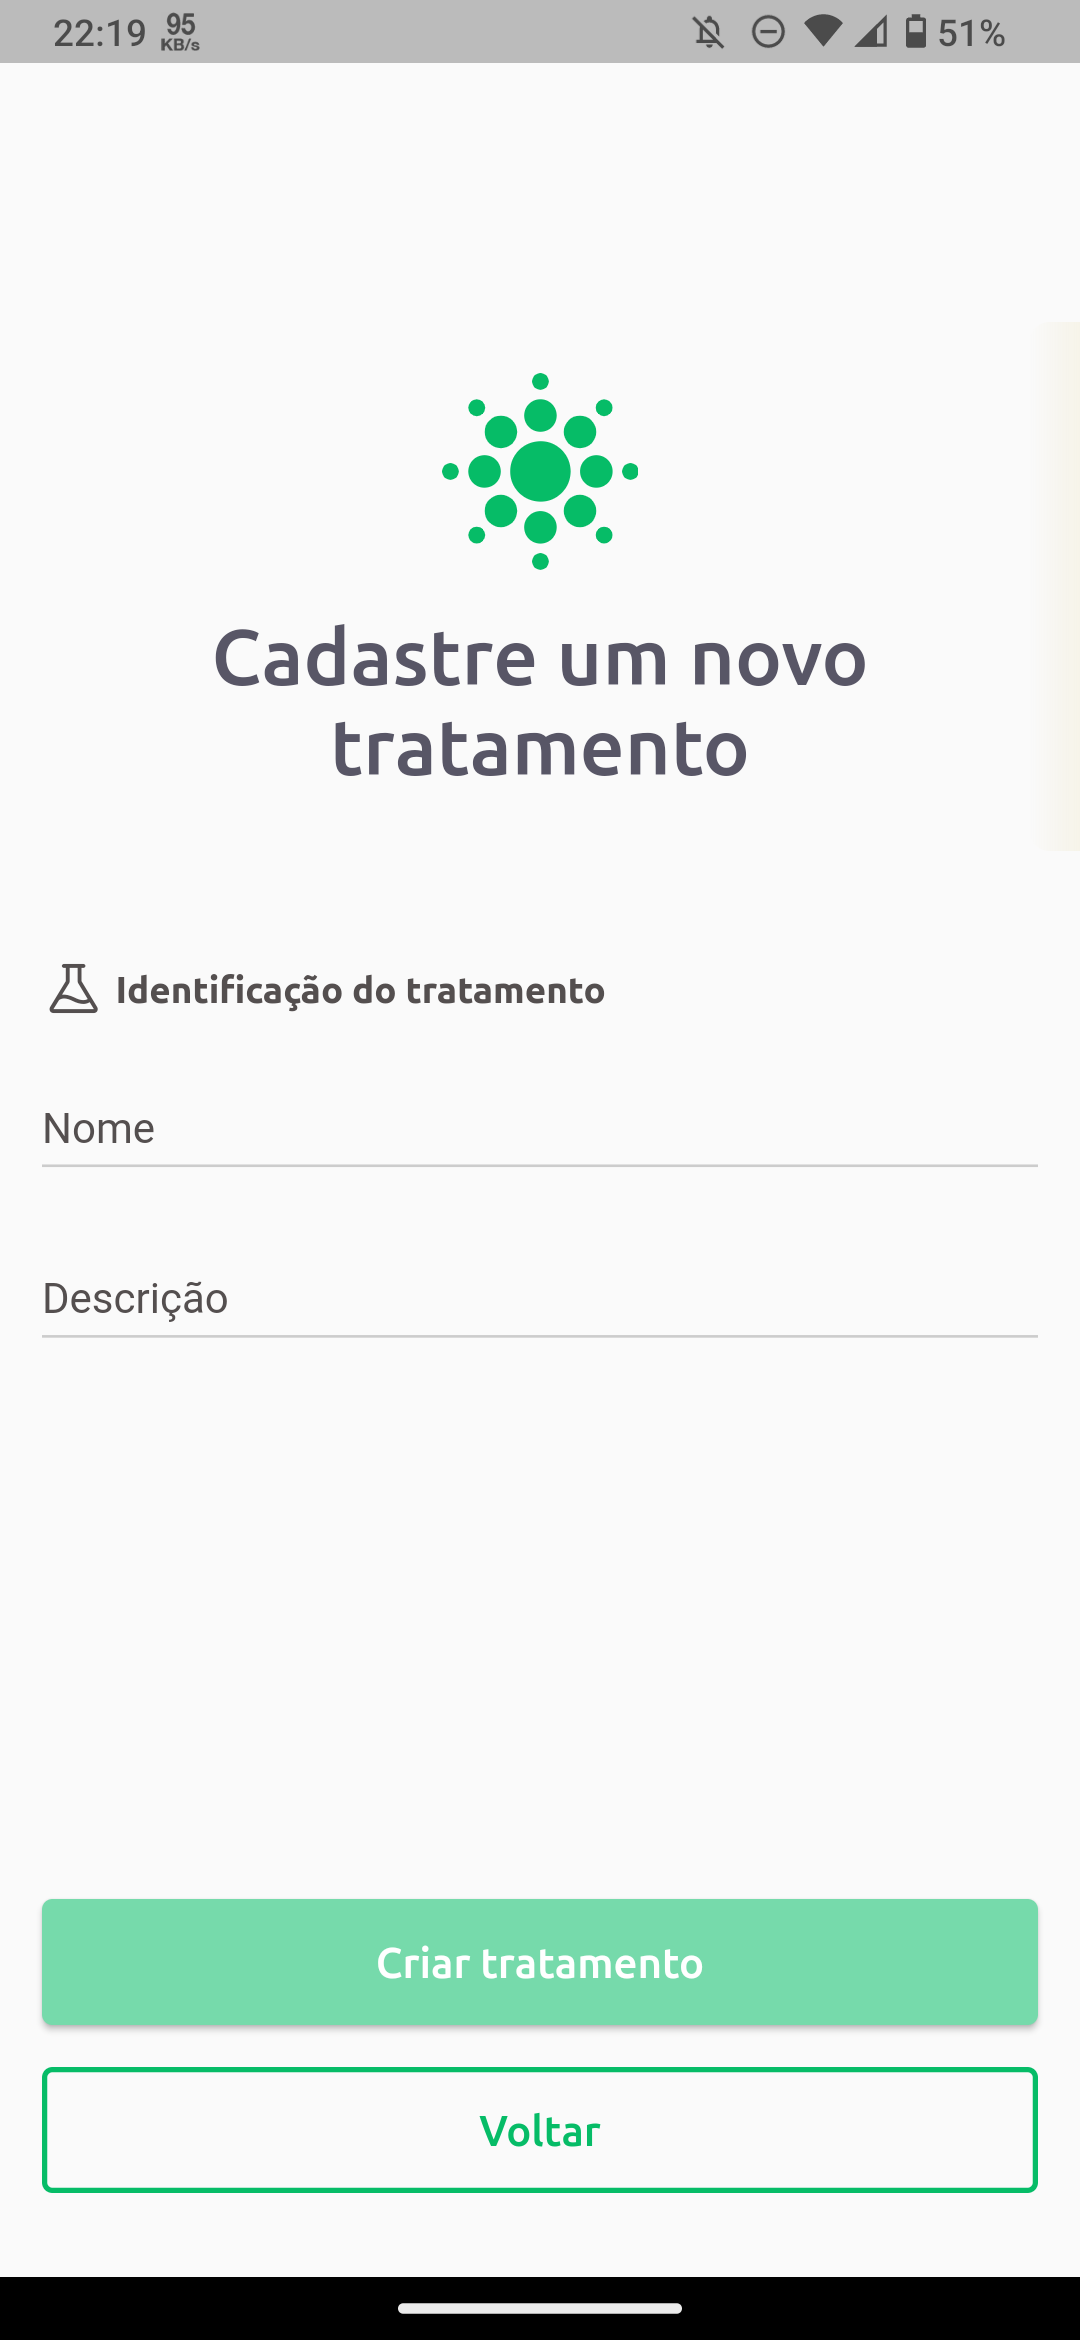
\includegraphics[width=.4\textwidth]{images/enzitech/cria_tratamento.png}\hfill
\caption{Fluxo de listagem, exclusão e criação de tratamentos}
\acsfont{Fonte: Aplicativo Enzitech desenvolvido pelo autor}
\label{fig:fluxo_tratamento}
\end{figure}

Após criado pelo menos uma enzima e um tratamento, o usuário consegue criar seu primeiro experimento, como mostrado no fluxo da \figref{fig:fluxo_cria_experimento} abaixo.

\begin{figure}[p]
  \centering
  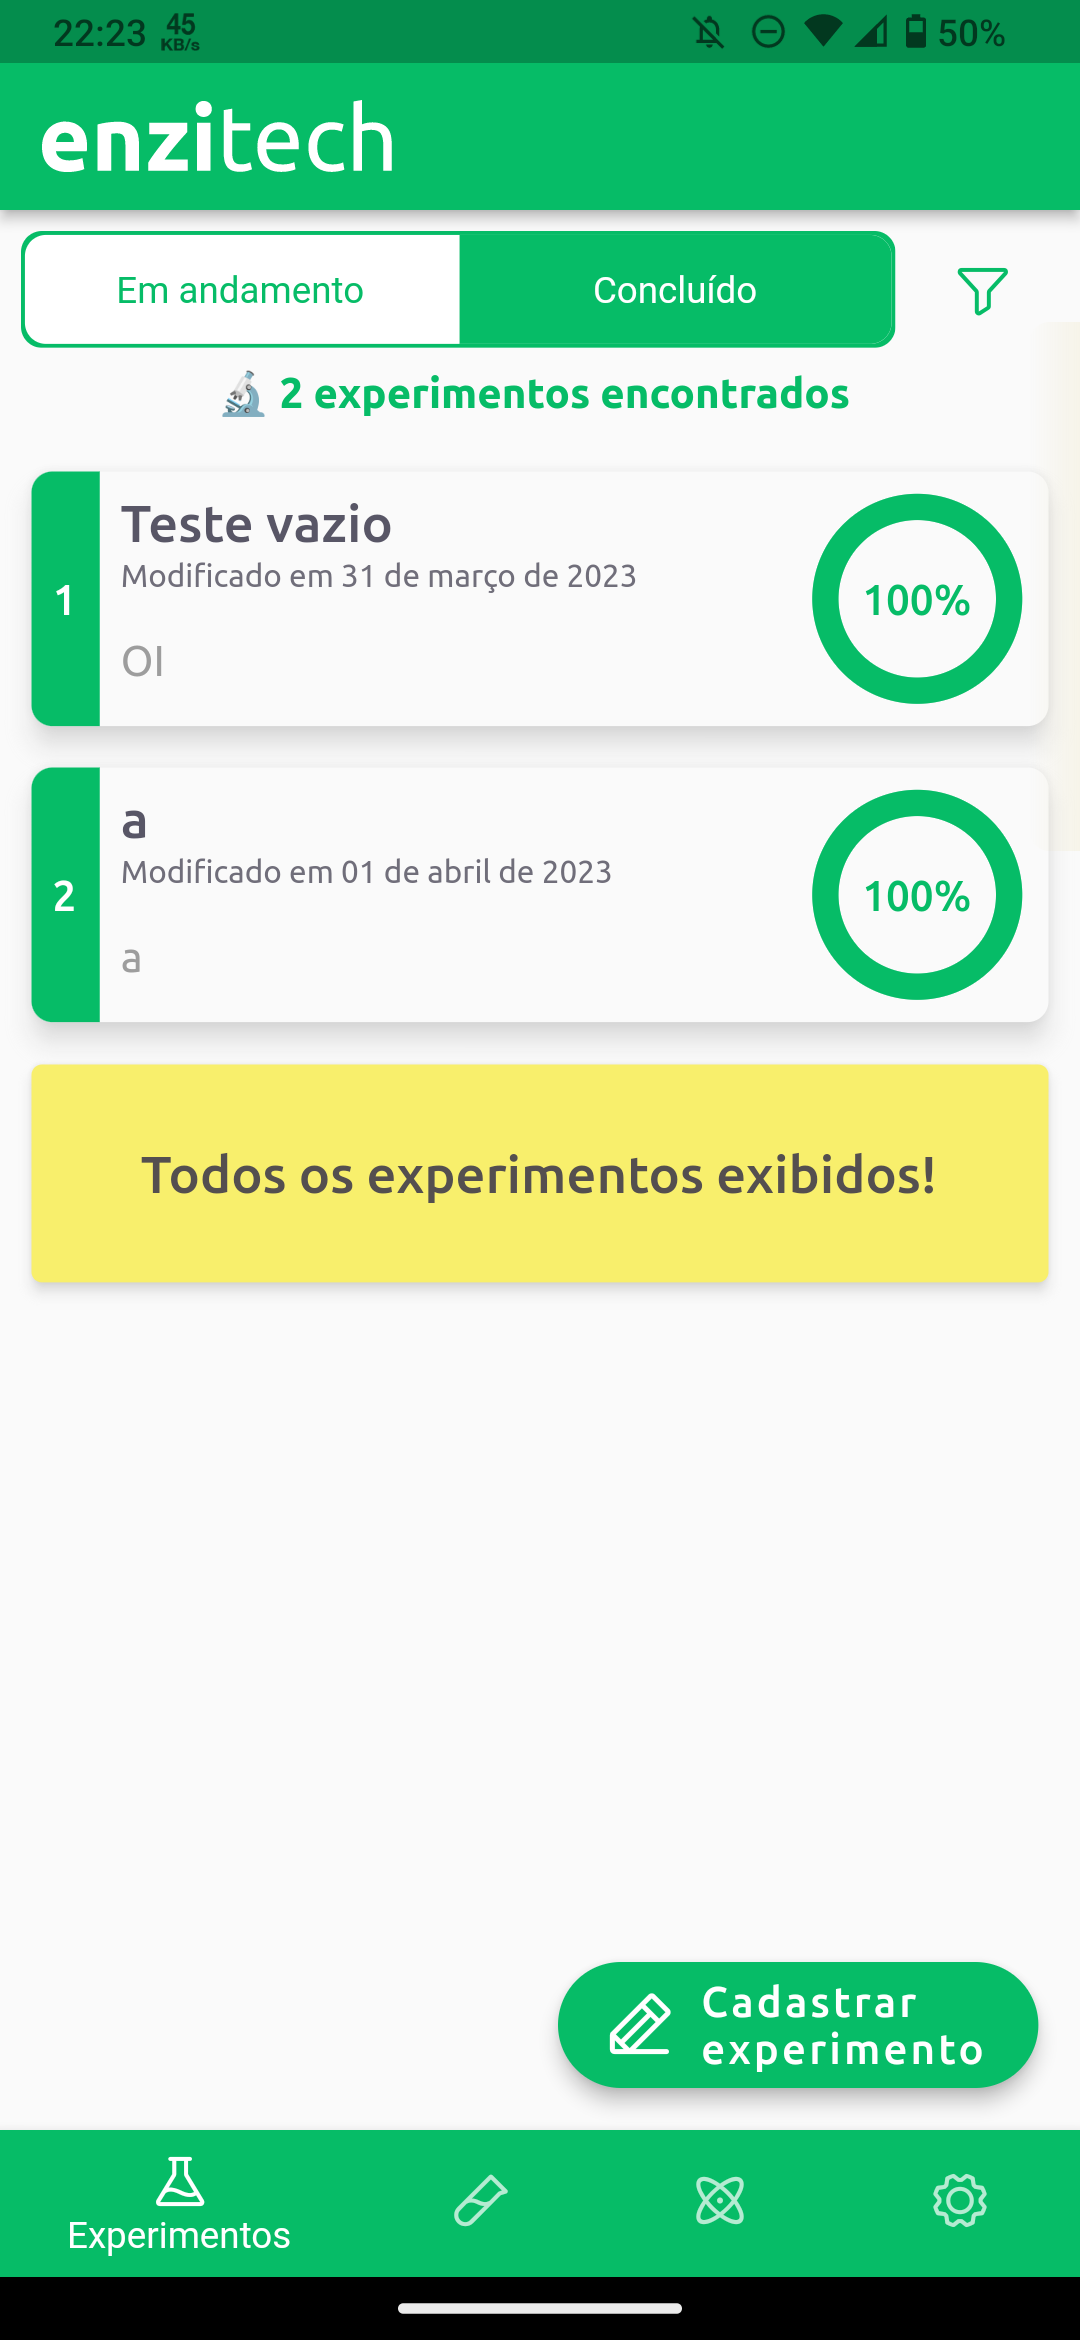
\includegraphics[width=.3\textwidth]{images/enzitech/home_2.png}
  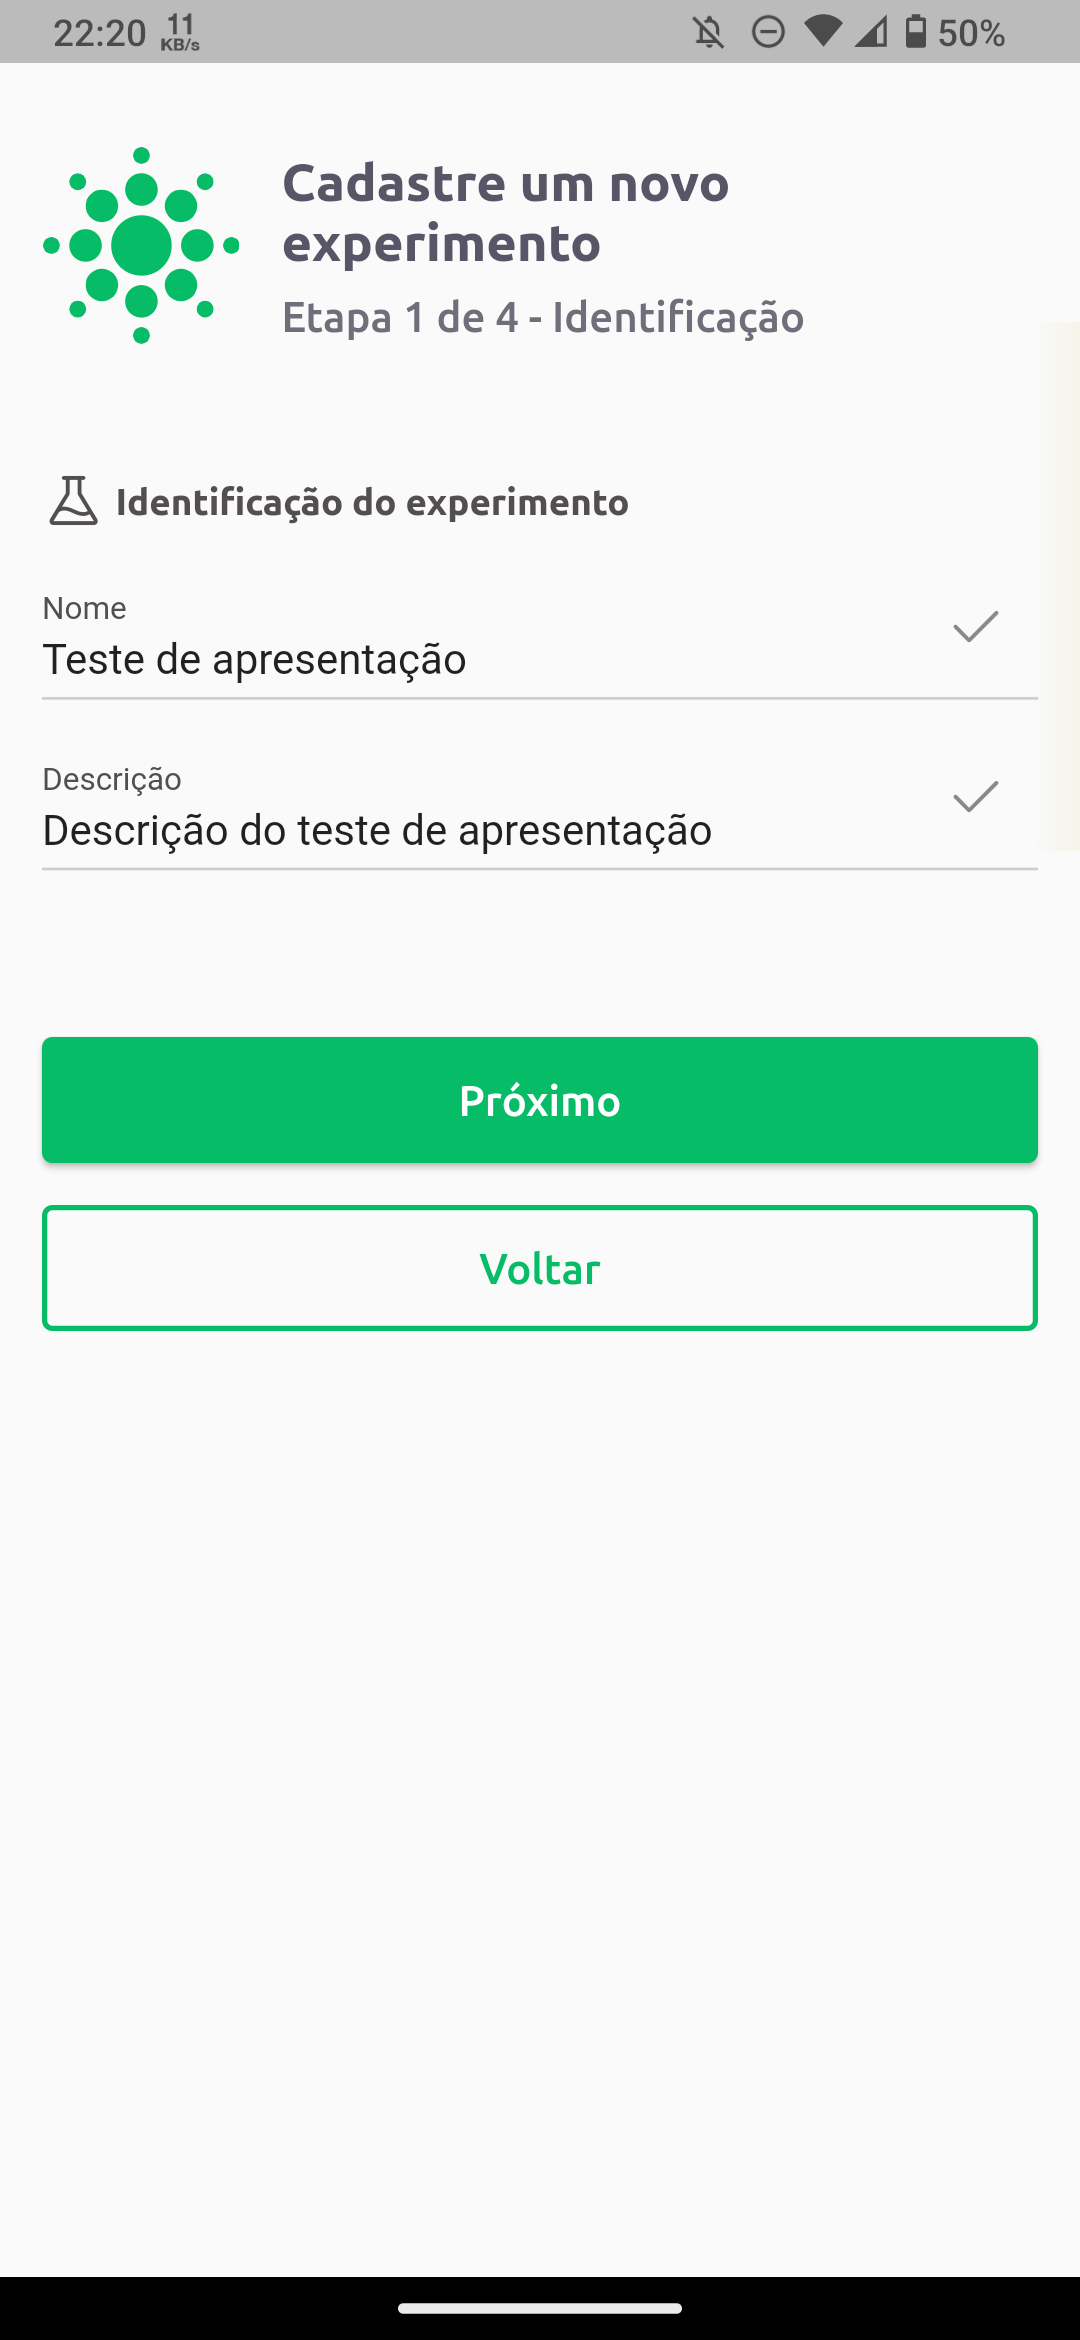
\includegraphics[width=.3\textwidth]{images/enzitech/cria_exp_1.png}
  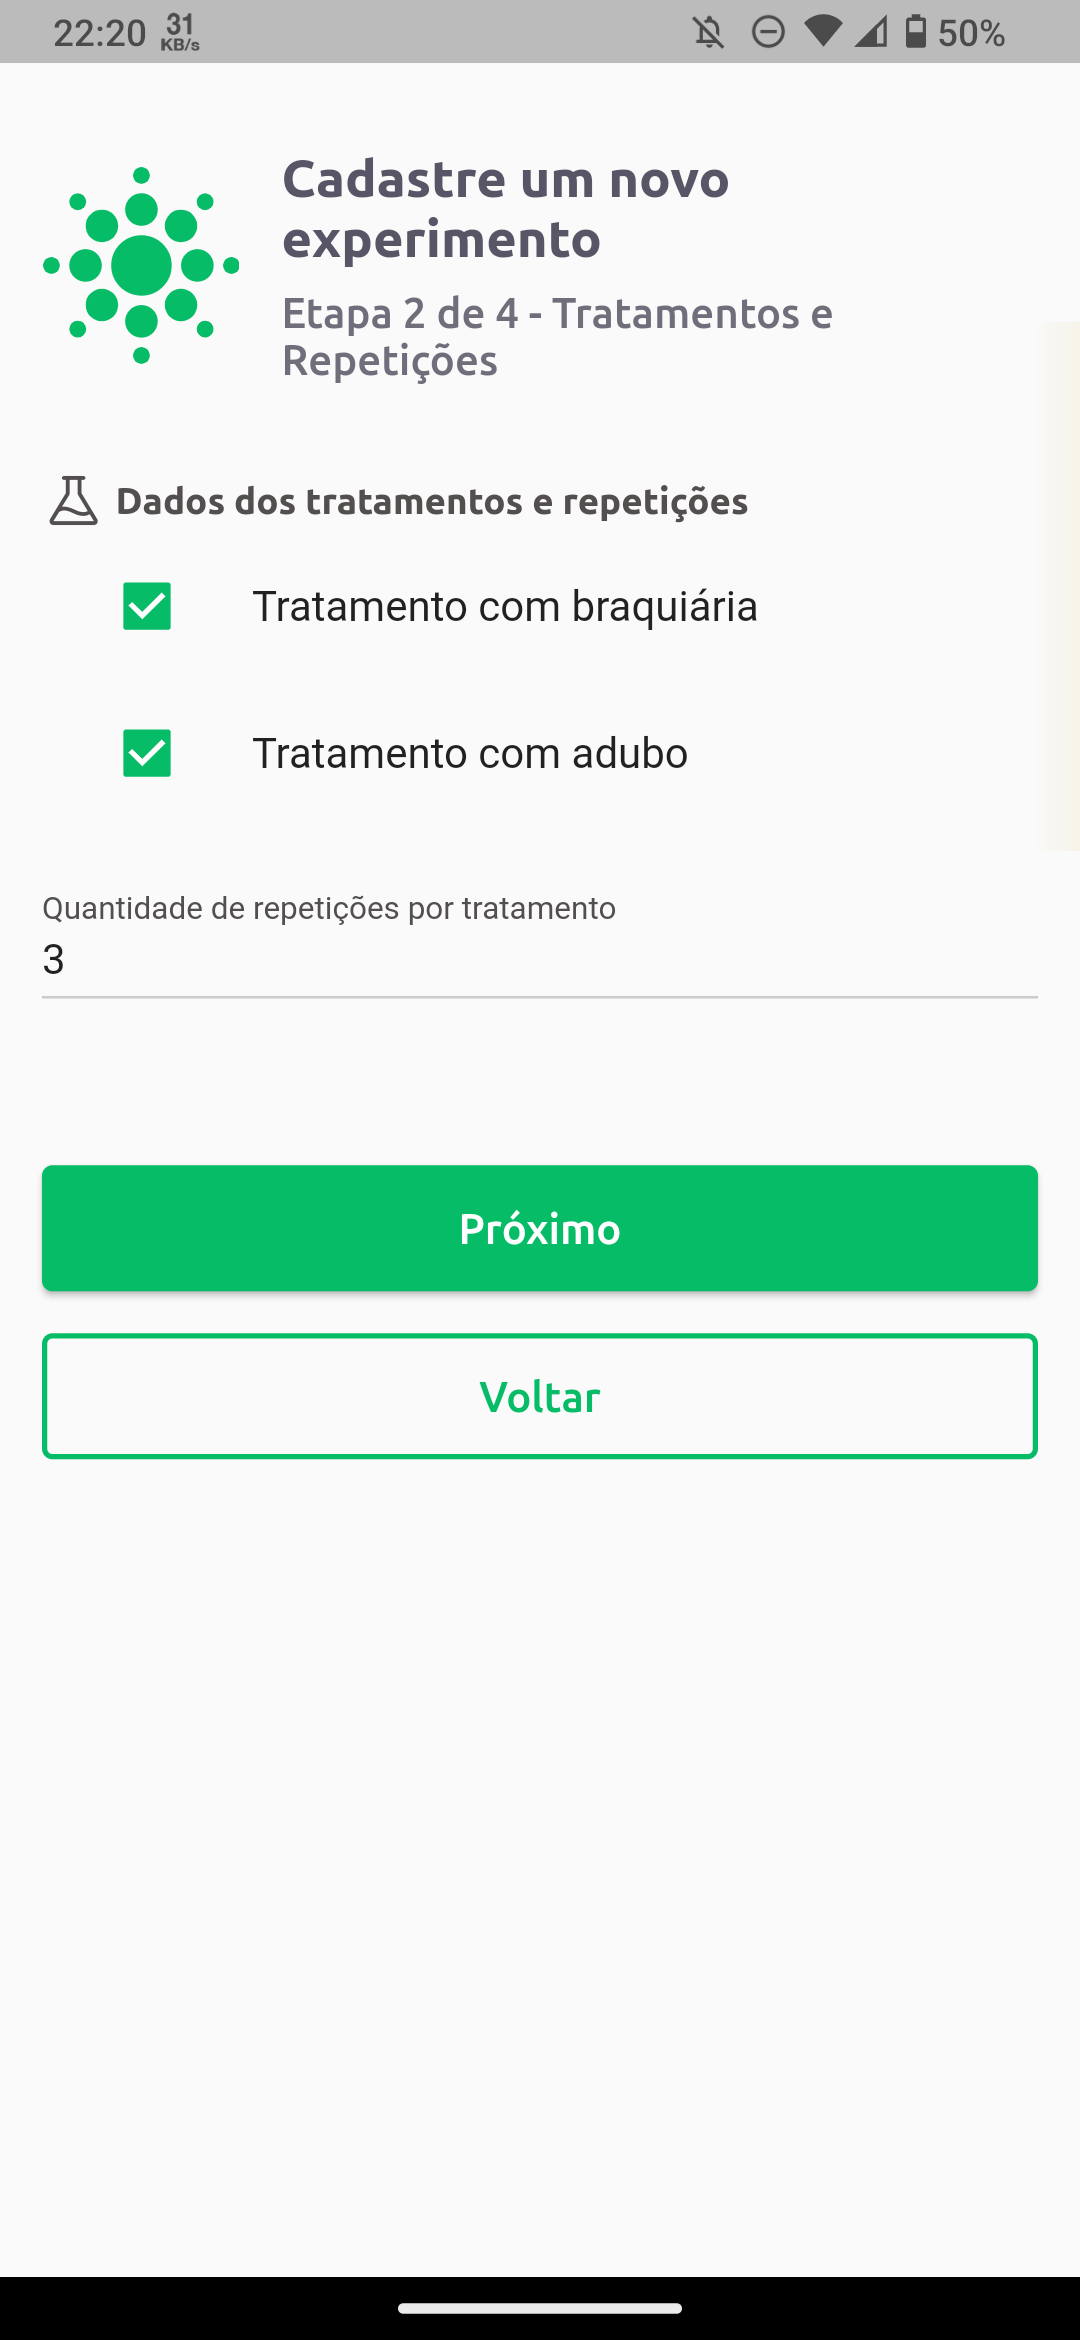
\includegraphics[width=.3\textwidth]{images/enzitech/cria_exp_2.png}

  \vspace{1cm}

  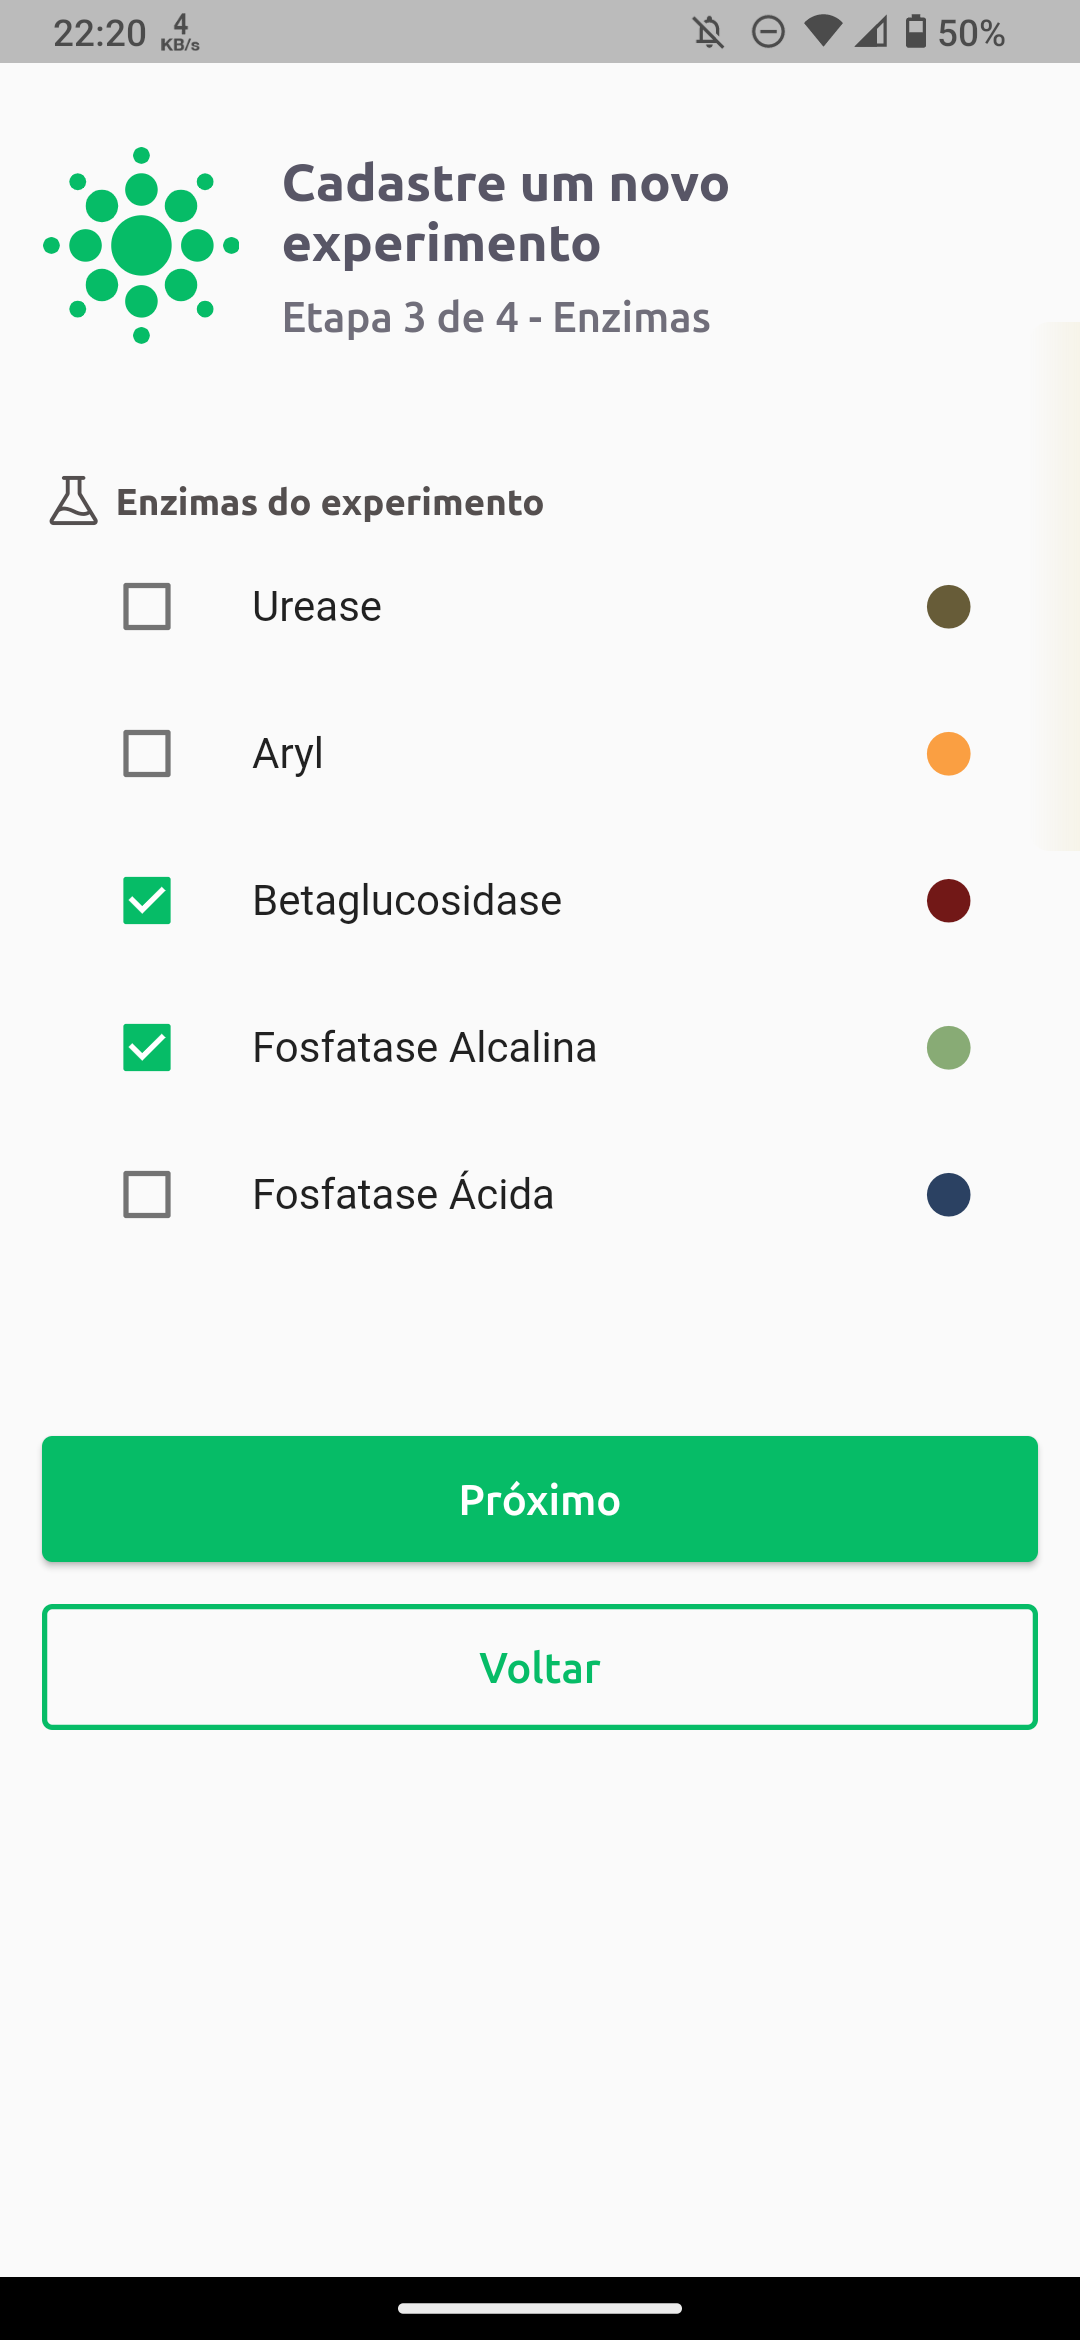
\includegraphics[width=.3\textwidth]{images/enzitech/cria_exp_3.png}
  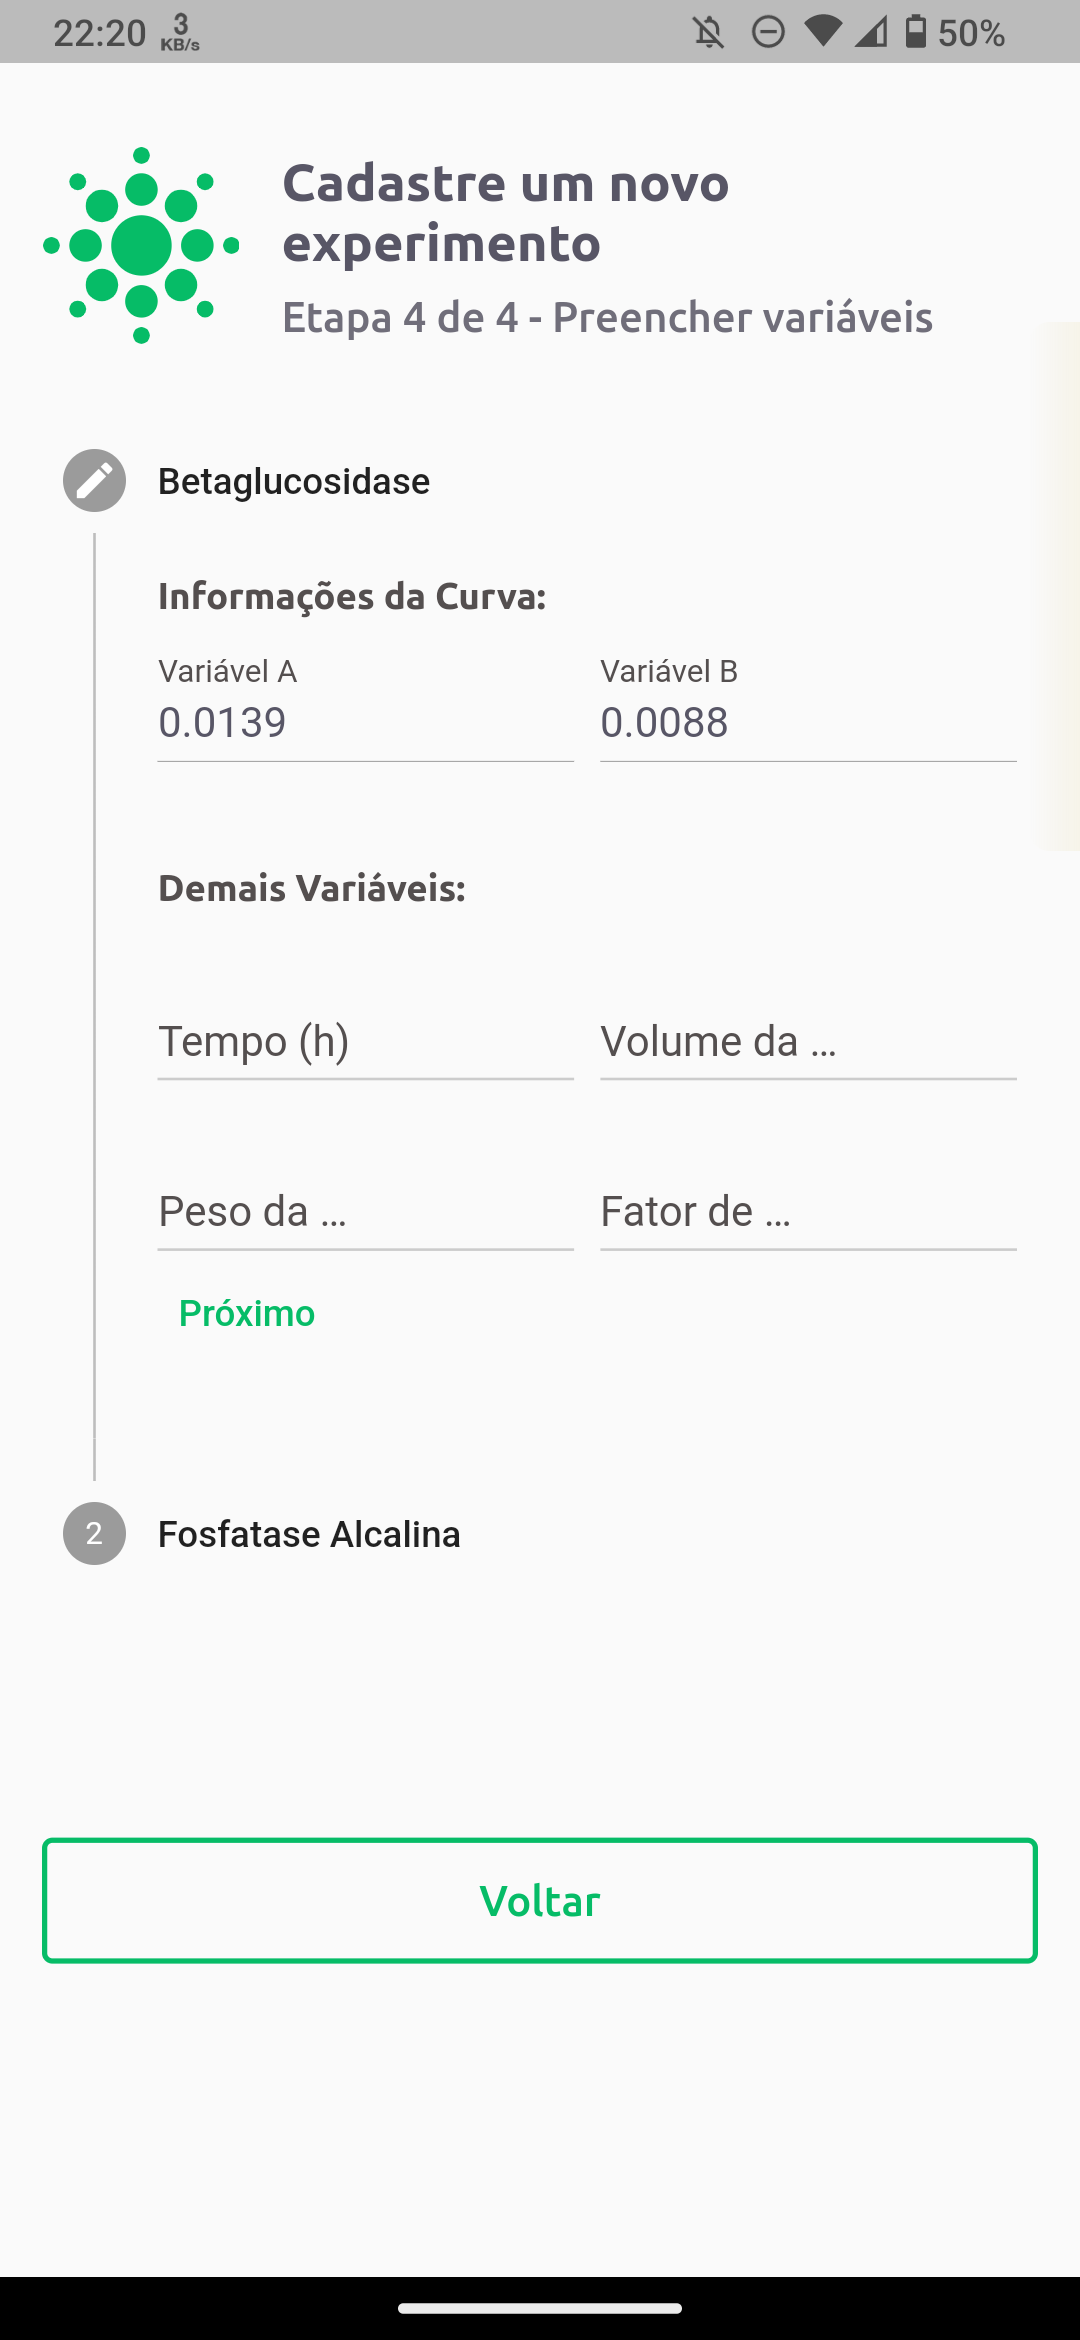
\includegraphics[width=.3\textwidth]{images/enzitech/cria_exp_4.png}
  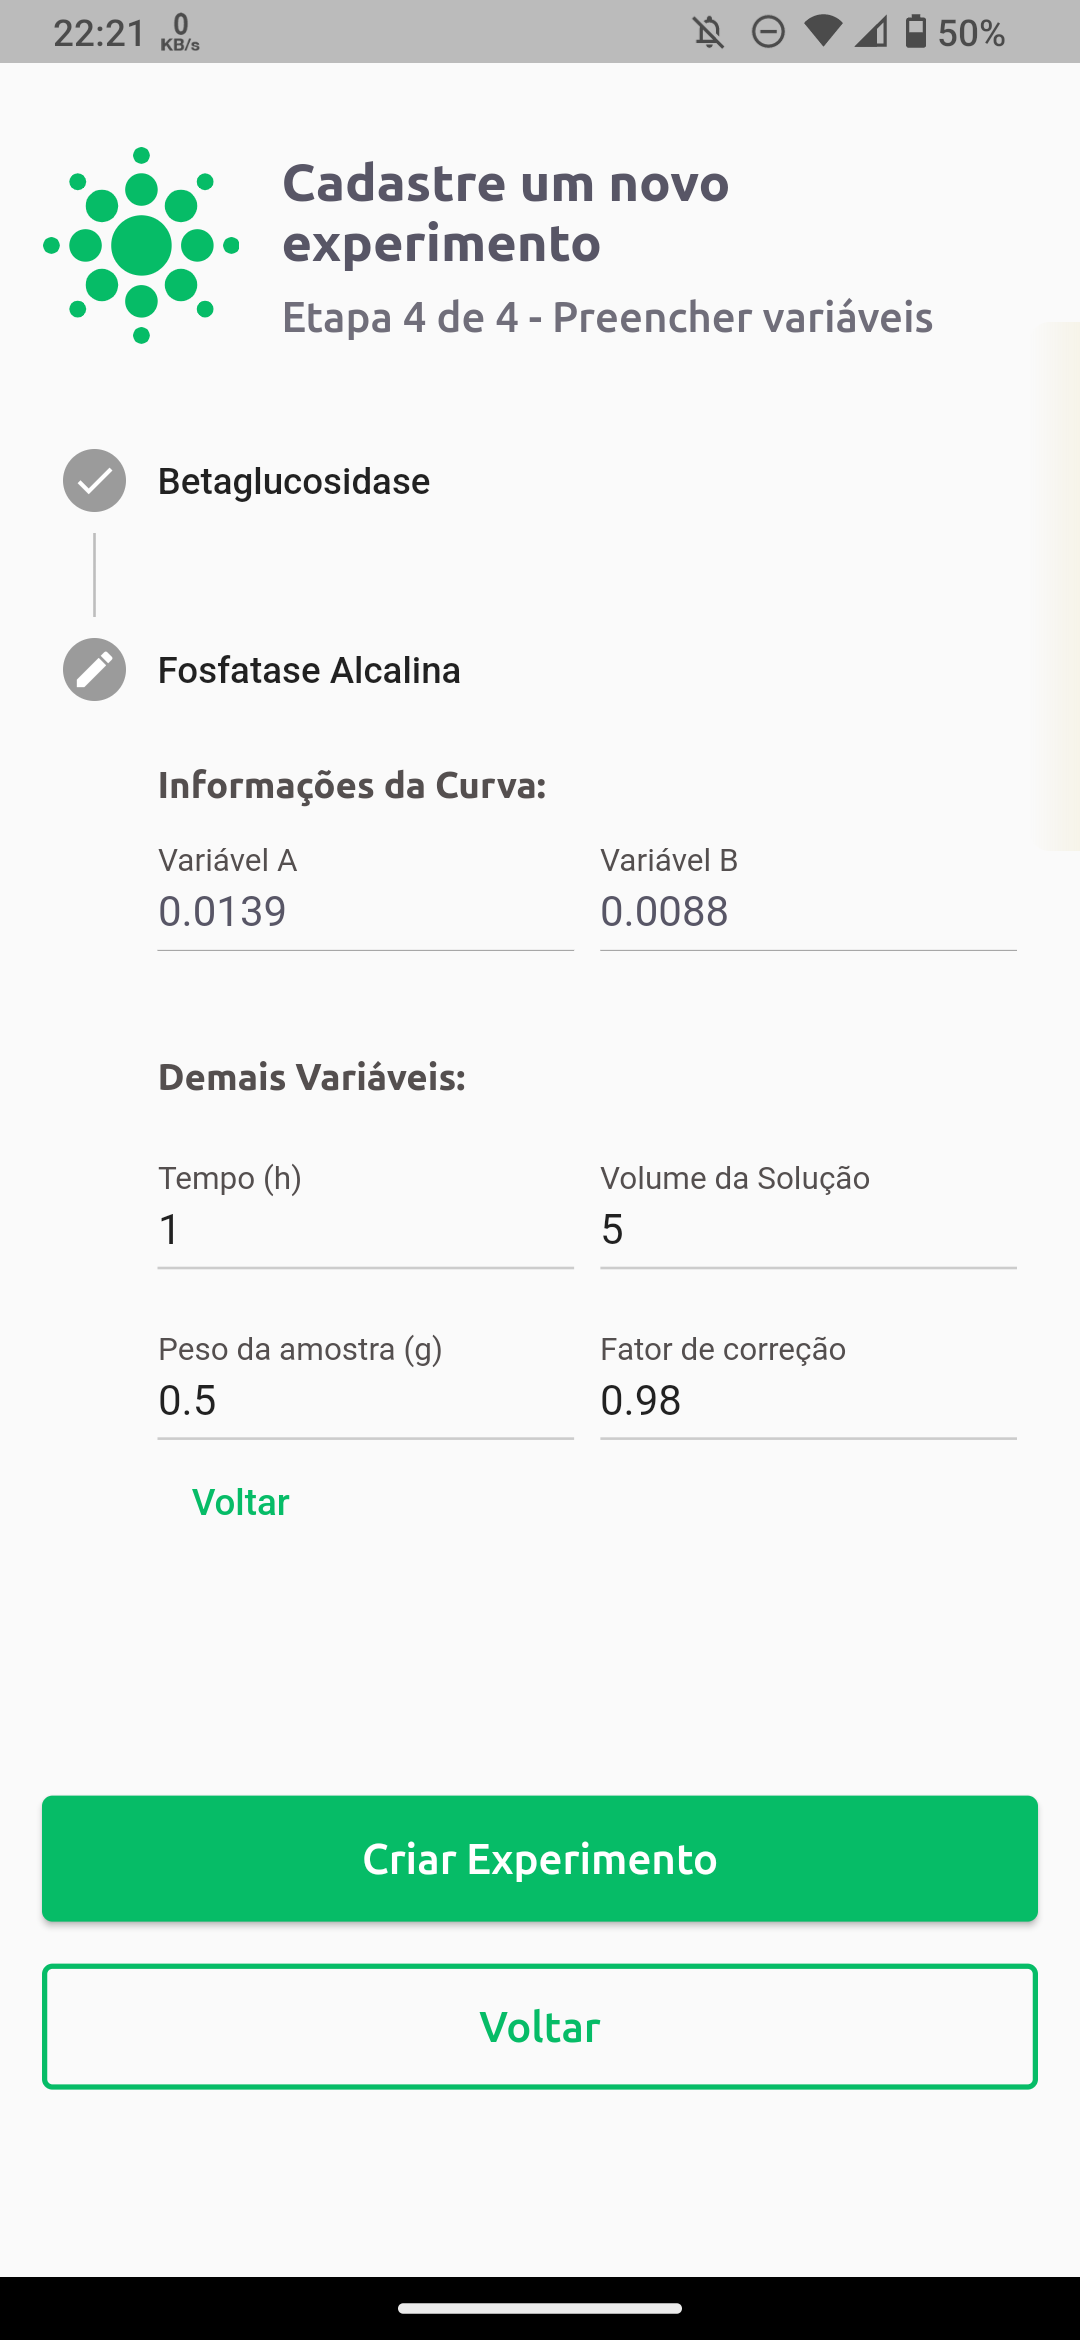
\includegraphics[width=.3\textwidth]{images/enzitech/cria_exp_5.png}

  \caption{Fluxo de criação de um experimento}
  \label{fig:fluxo_cria_experimento}
  \acsfont{Fonte: Aplicativo Enzitech desenvolvido pelo autor}
  
\end{figure}


É possível ver na primeira imagem, na tela de experimentos, o filtro de "experimentos concluídos" aplicado, seguindo o fluxo, na segunda imagem é solicitada as informações de identificação do experimento, nome e descrição, a seguir, os tratamentos daquele experimento e quantas repetições serão realizadas, logo após, surge o seletor de enzimas, na quarta imagem (terceira etapa do processo de criação de experimento), nele é possível escolher quais enzimas farão parte do experimento, logo após surge a última etapa para o preenchimento dos valores variáveis daquele experimento, após criado (concluindo o caso de uso UC07), o usuário é levado para a funcionalidade de visualizar o experimento, explicado na \figref{fig:fluxo_experimento_detalhado} a seguir.

\begin{figure}[p]
  \centering
  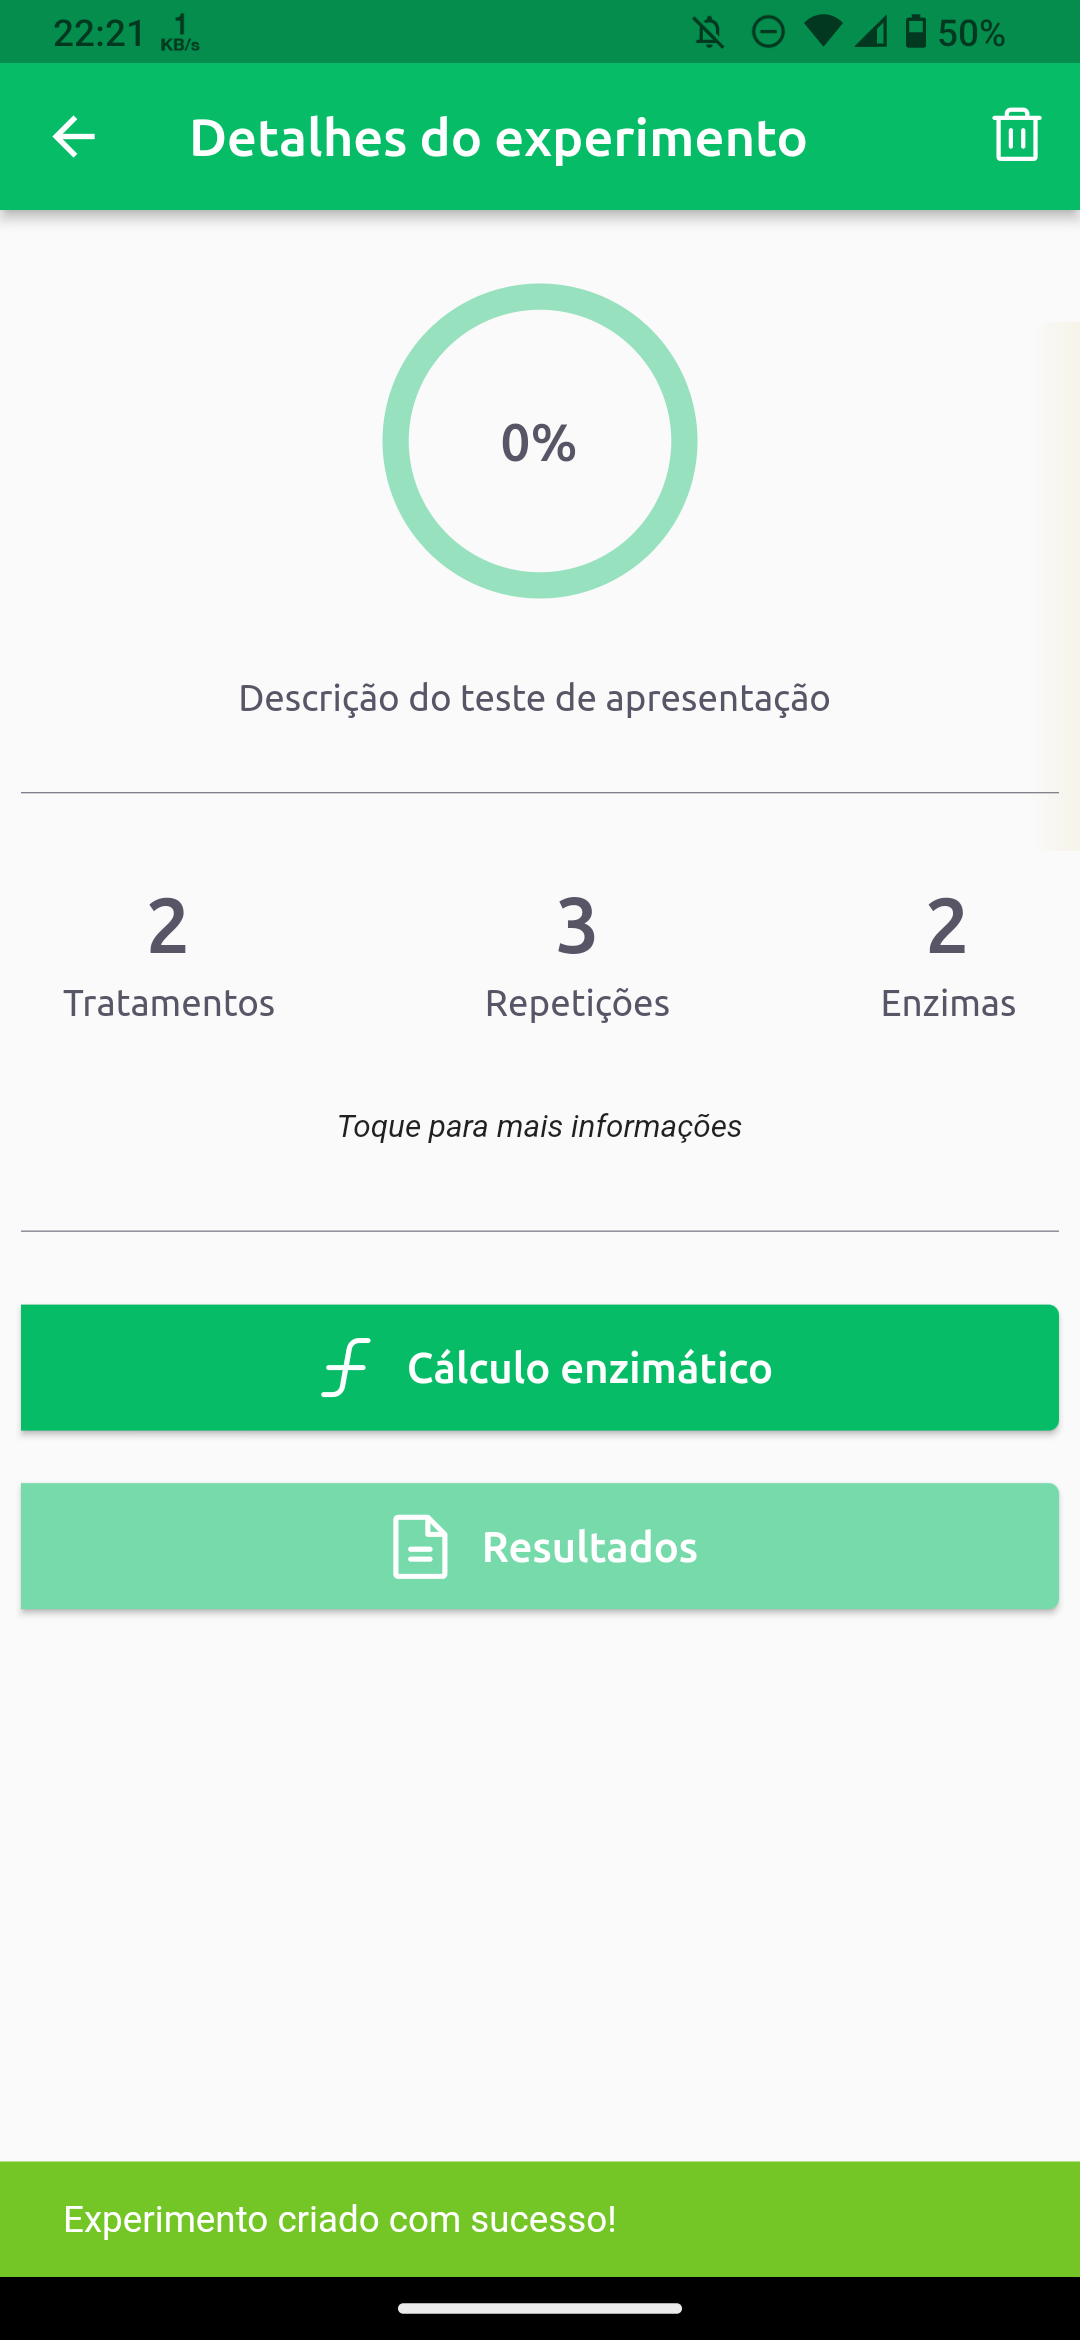
\includegraphics[width=.3\textwidth]{images/enzitech/exp_detalhado.png}
  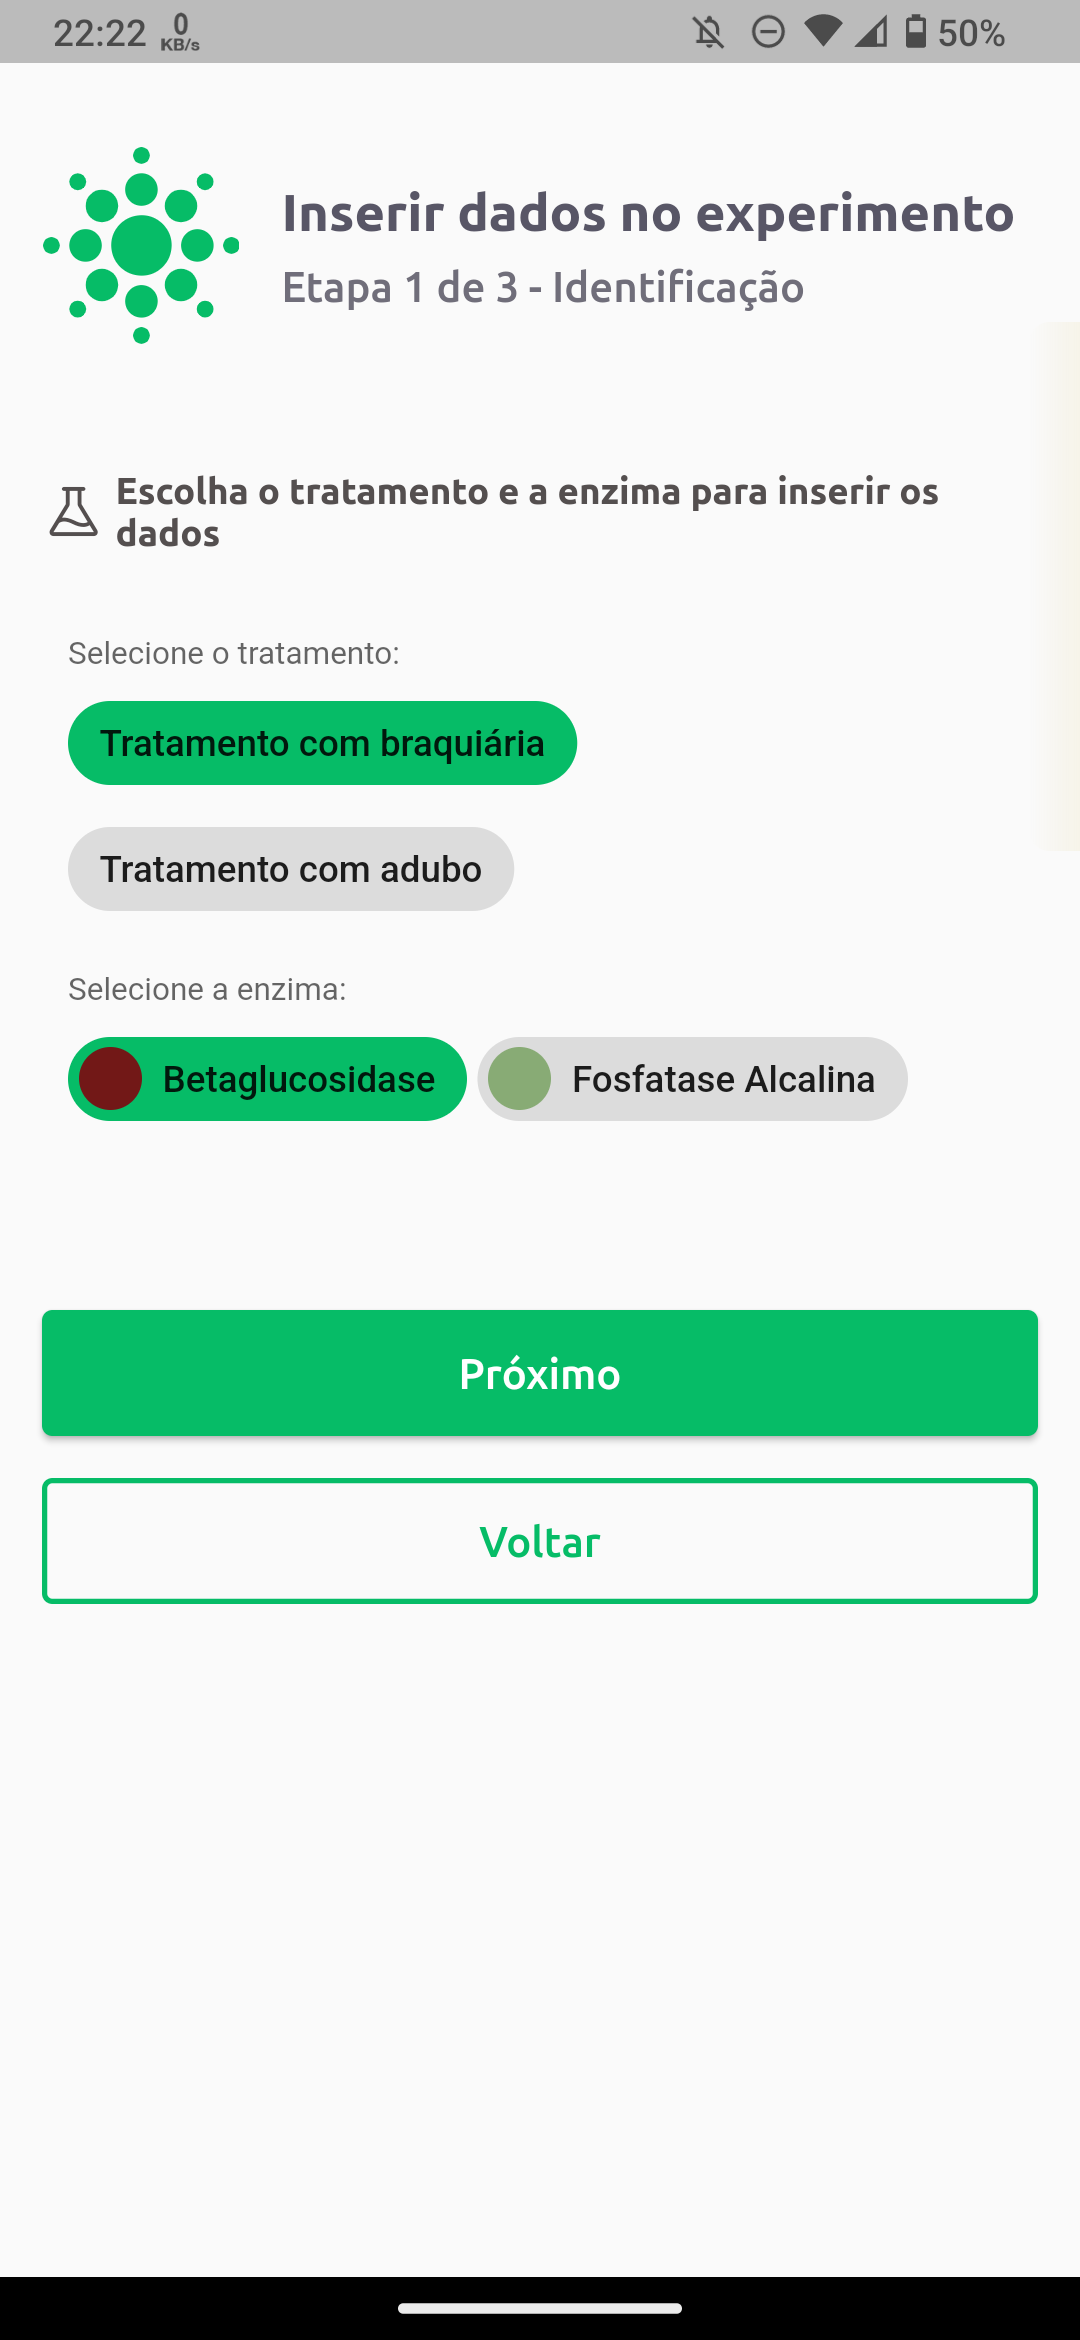
\includegraphics[width=.3\textwidth]{images/enzitech/calculo_1.png}
  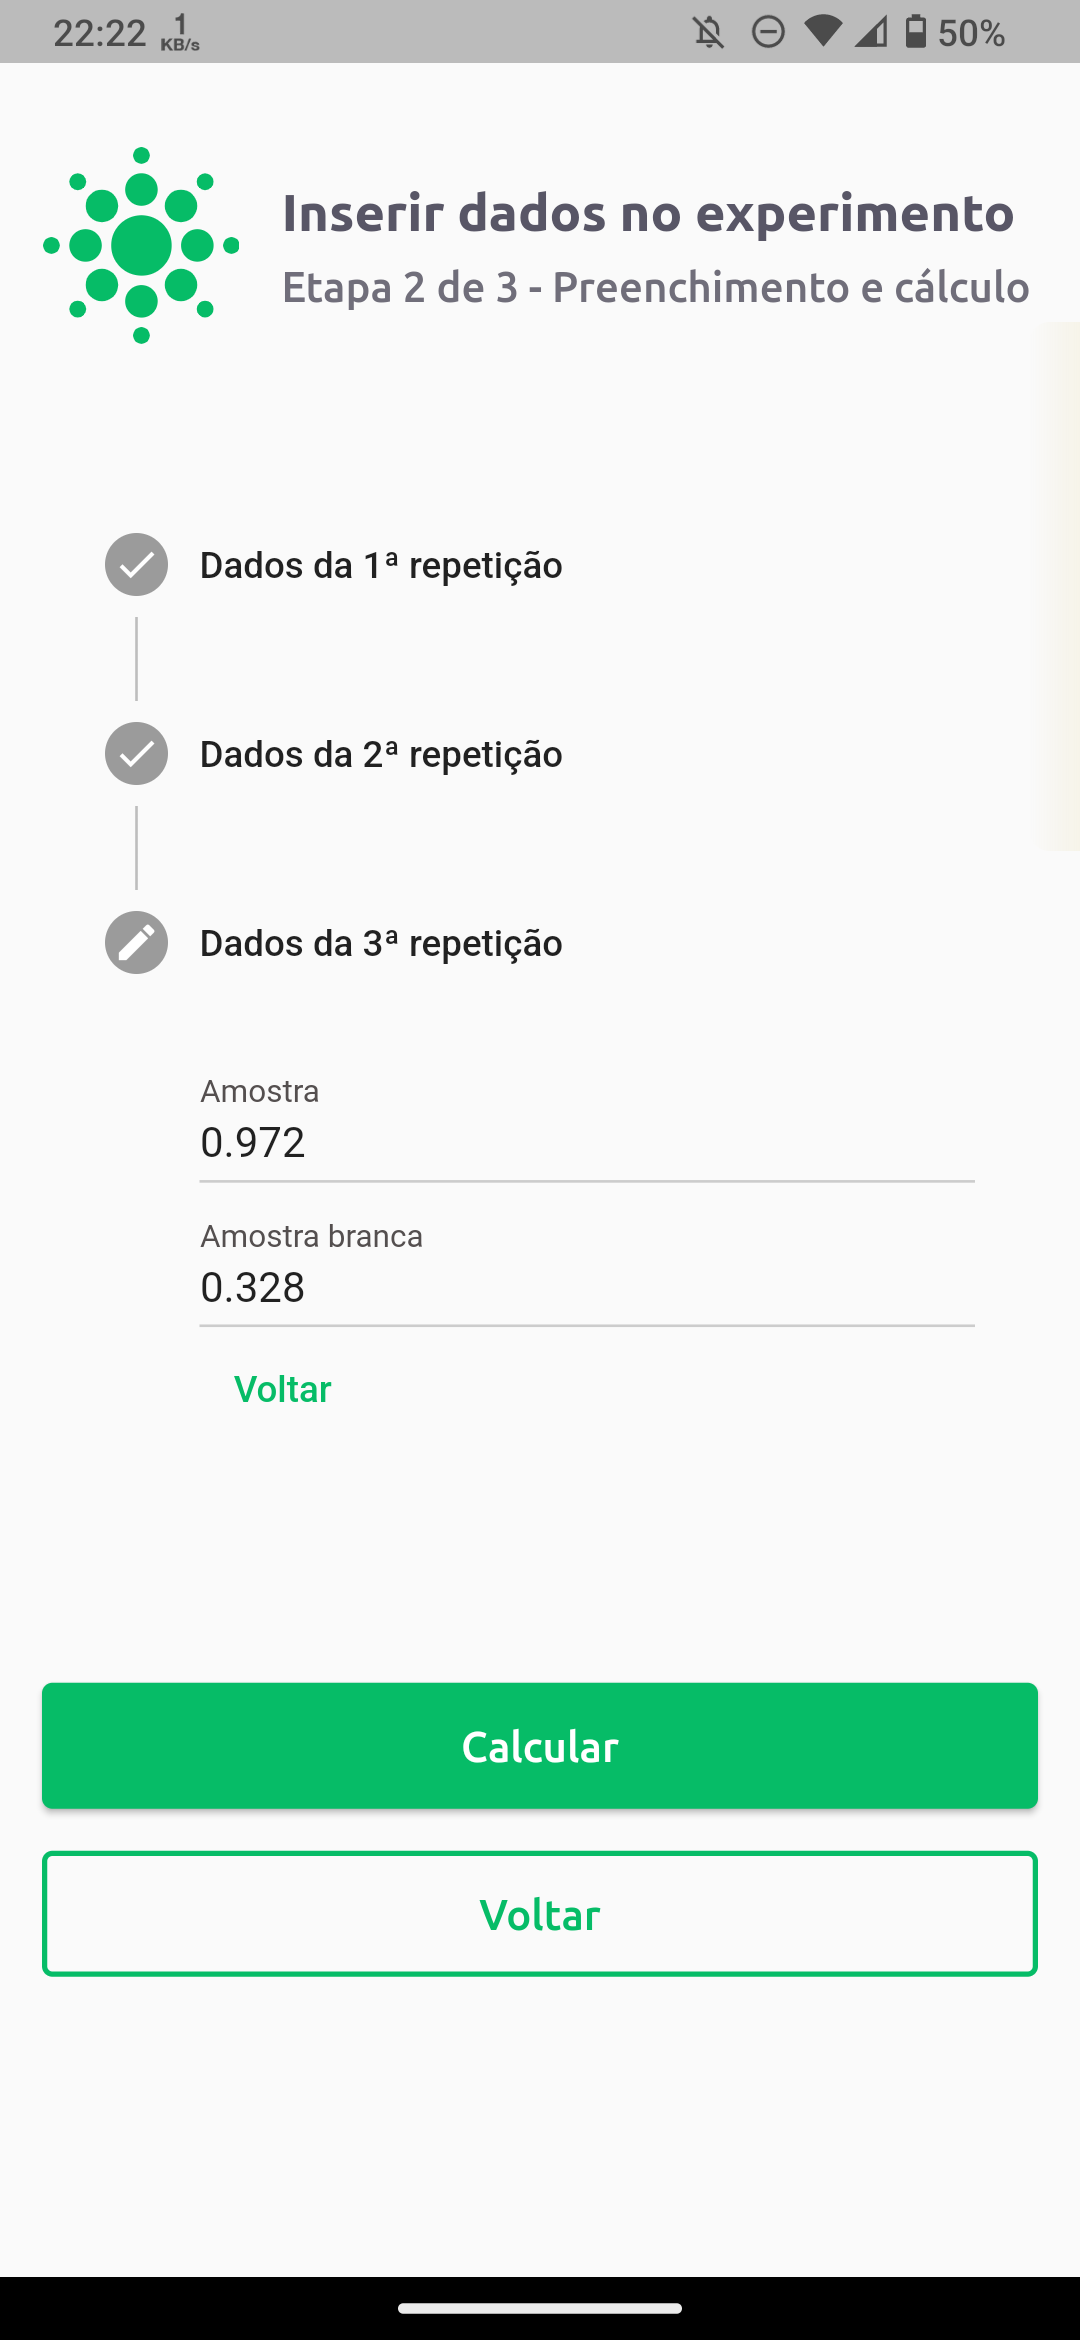
\includegraphics[width=.3\textwidth]{images/enzitech/calculo_2.png}

  \vspace{1cm}

  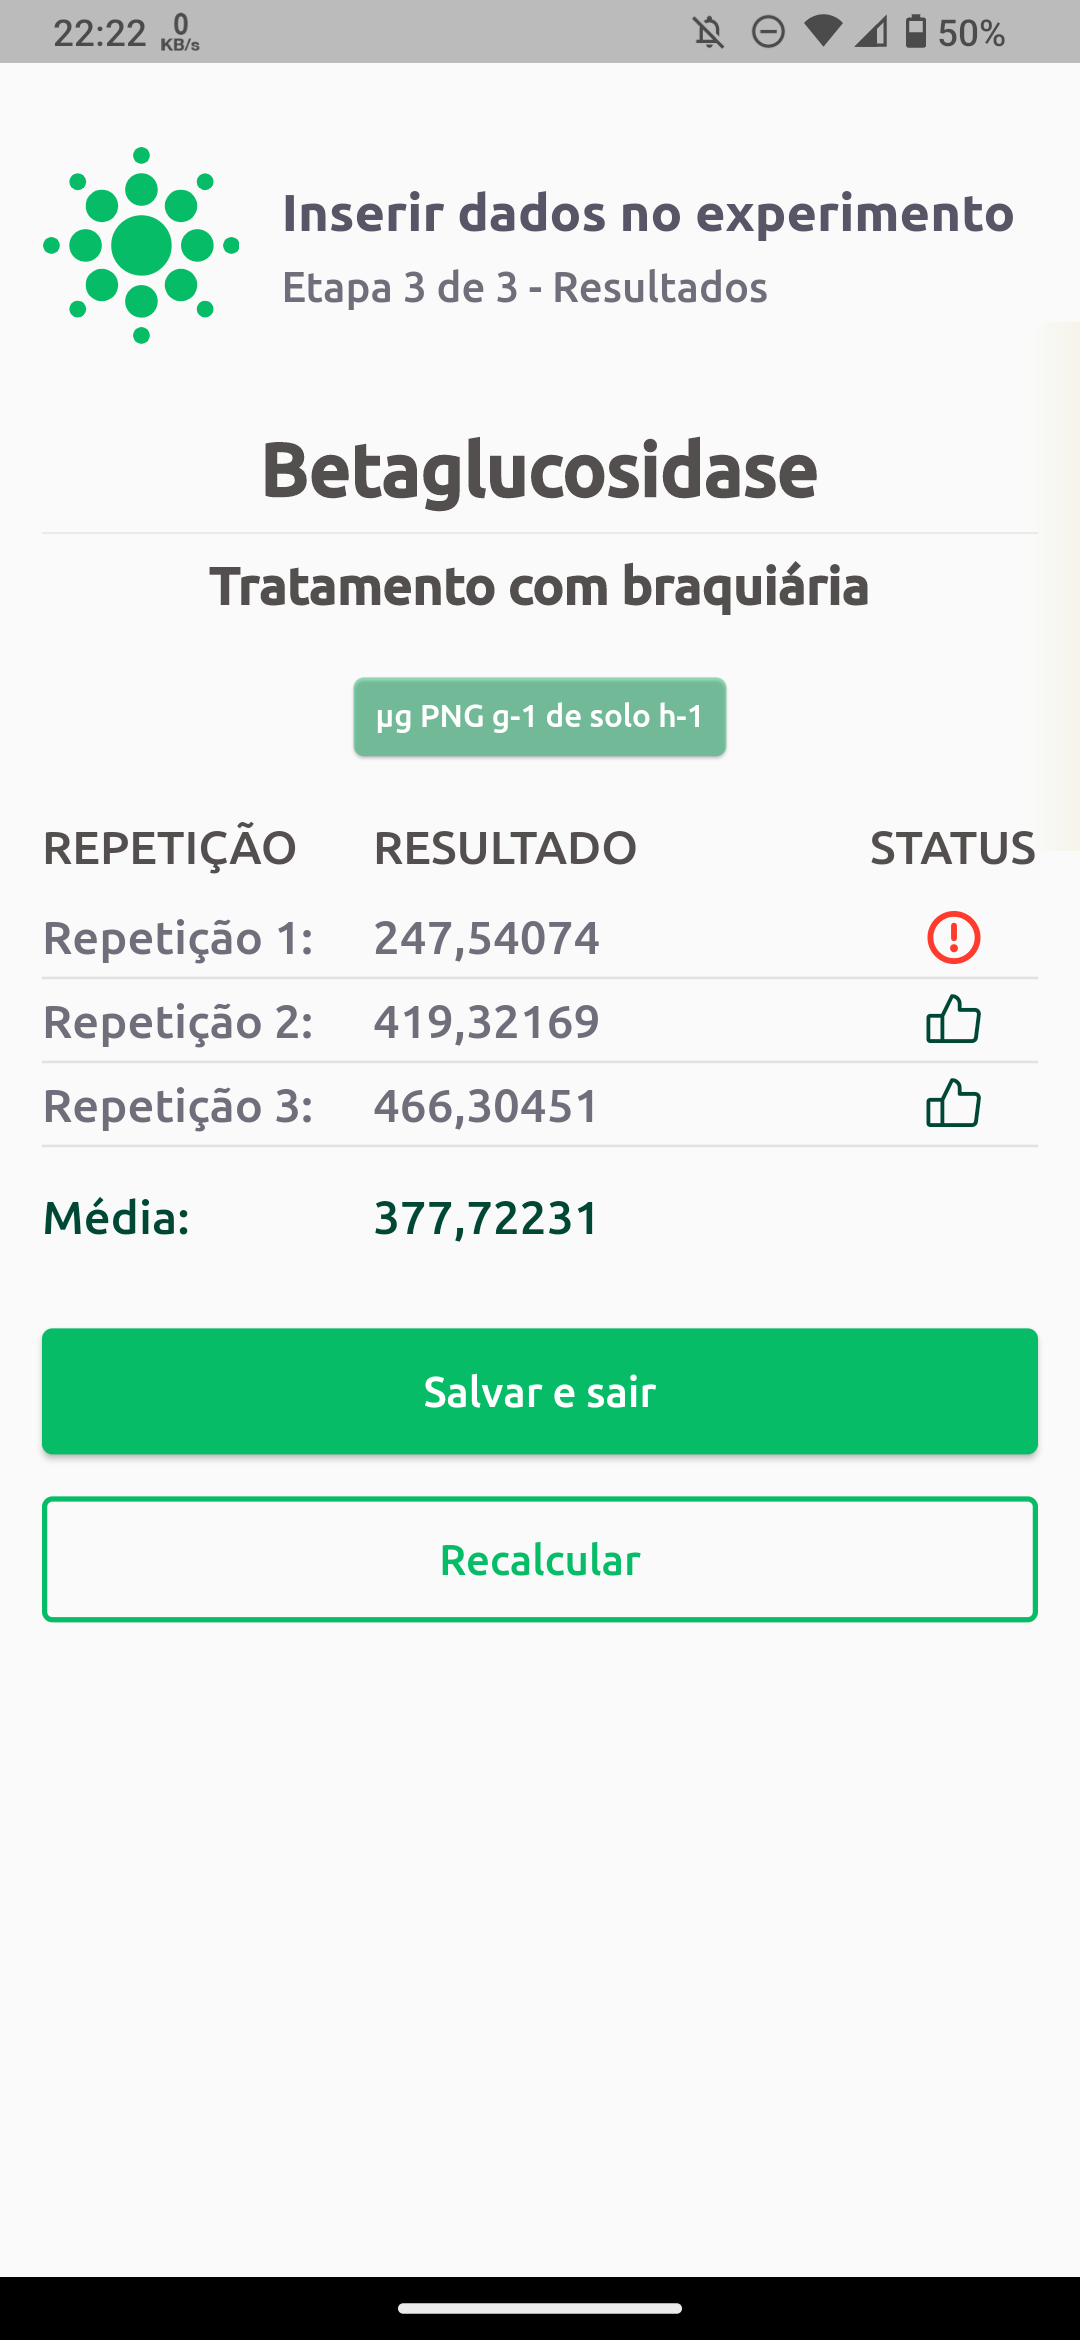
\includegraphics[width=.3\textwidth]{images/enzitech/calculo_3.png}
  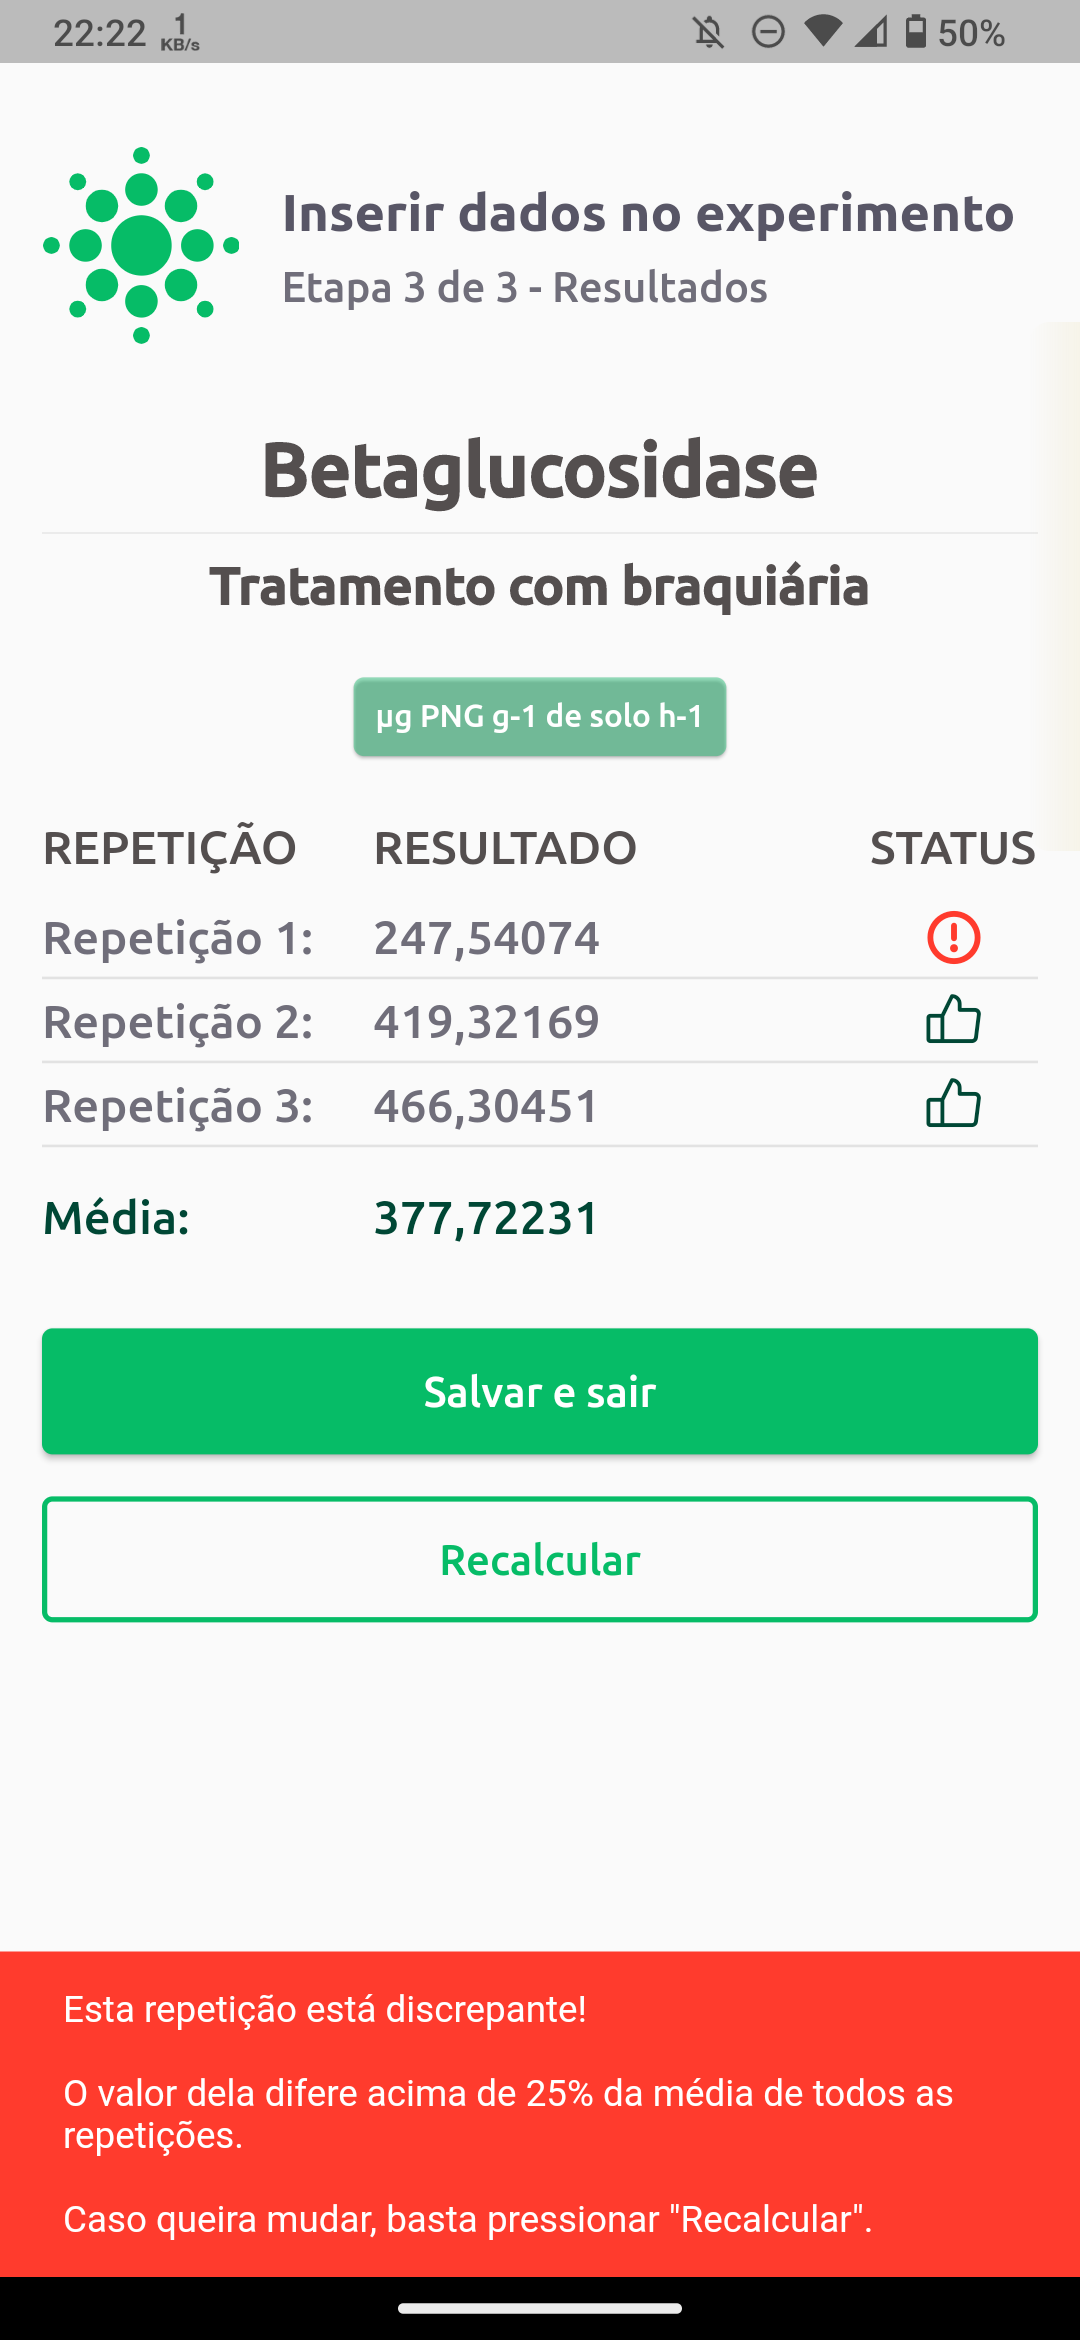
\includegraphics[width=.3\textwidth]{images/enzitech/calculo_4.png}
  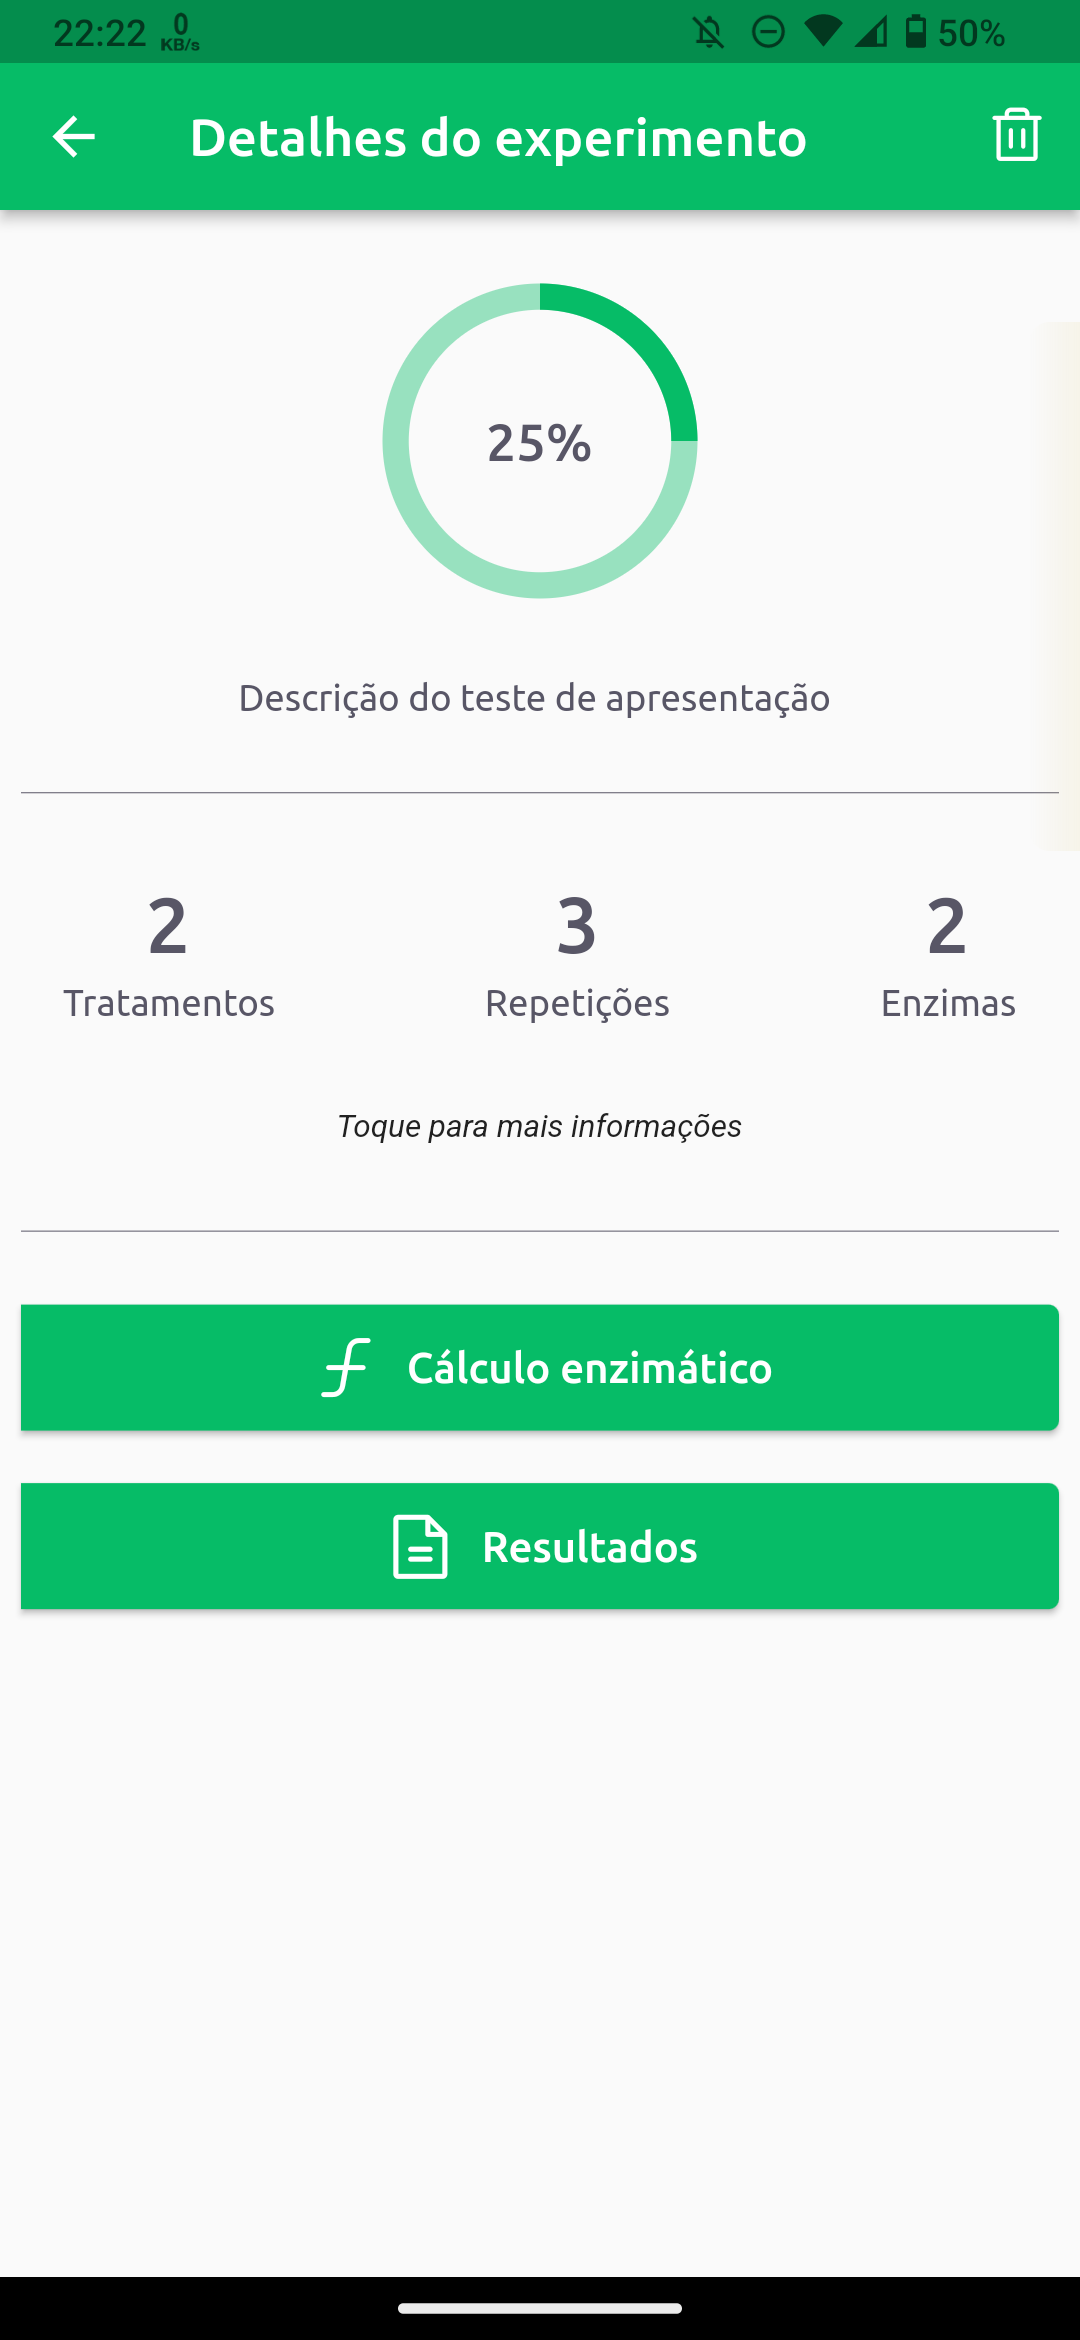
\includegraphics[width=.3\textwidth]{images/enzitech/exp_detalhado2.png}

  \caption{Fluxo de detalhamento e cálculo enzimático de um experimento}
  \label{fig:fluxo_experimento_detalhado}
  \acsfont{Fonte: Aplicativo Enzitech desenvolvido pelo autor}
  
\end{figure}

Após o experimento criado, o usuário pode ver seus detalhes, como a quantidade de enzimas, tratamentos e repetições, seu progresso (caso de uso UC08) e a possibilidade de excluí-lo, além disso, o acesso à outras duas funcionalidades, a de cálculo enzimático, para inserção de dados no experimento, e a de resultados, para a visualização e compartilhamento desses dados também estão contidos nesta tela, todas elas serão explicadas a seguir.

Acompanhando novamente a \figref{fig:fluxo_experimento_detalhado}, para o preenchimento do experimento é necessário escolher um tratamento e uma enzima, assim, gerando um conjunto de informações para prosseguir com a inserção dos valores em suas respectivas repetições, após todos os valores inseridos, o usuário clica em carregar e é levado para uma tela de resultados deste cálculo e a média (quarta e quinta imagem), nesta tela, é possível ver os resultados e receber um \textit{feedback} sobre a discrepância dos valores em comparação com a média de todos os resultados das repetições, assim, sendo possível perceber algum valor que pode estar inserido incorretamente, resultando em dados errôneos, desta forma, o usuário pode recalcular, corrigindo com novos valores ou prosseguir, salvando e saindo da tela de cálculo (caso de uso UC09).

Em seguida, quando um experimento já tem dados suficientes (progresso maior ou igual a 1\%), é possível ver e compartilhar os resultados obtidos (casos de uso UC10 e UC11), mostrados a seguir na \figref{fig:fluxo_resultados}.

\begin{figure}[p]
  \centering
  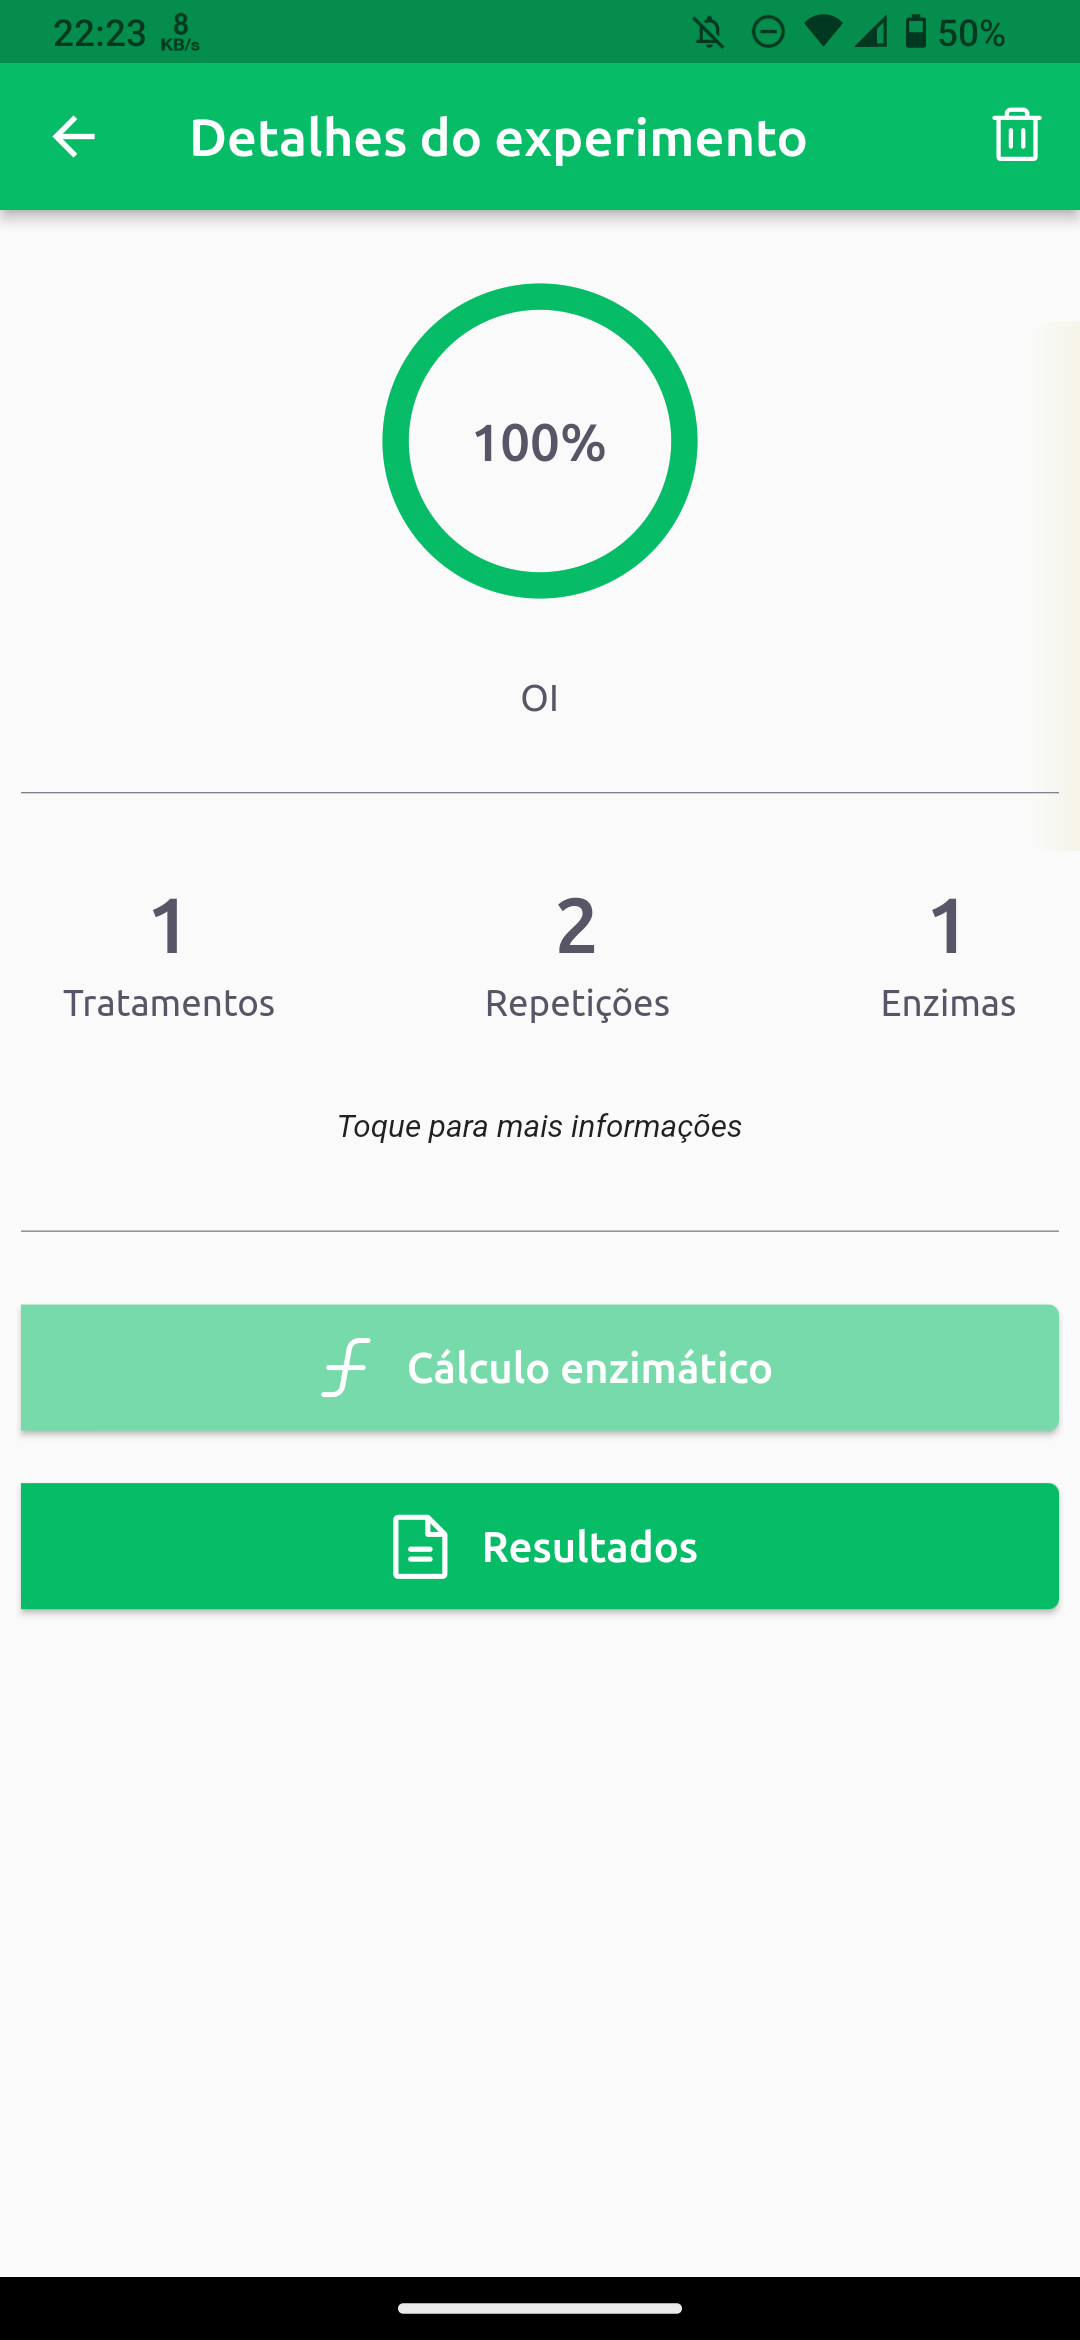
\includegraphics[width=.3\textwidth]{images/enzitech/exp_concluido.png}
  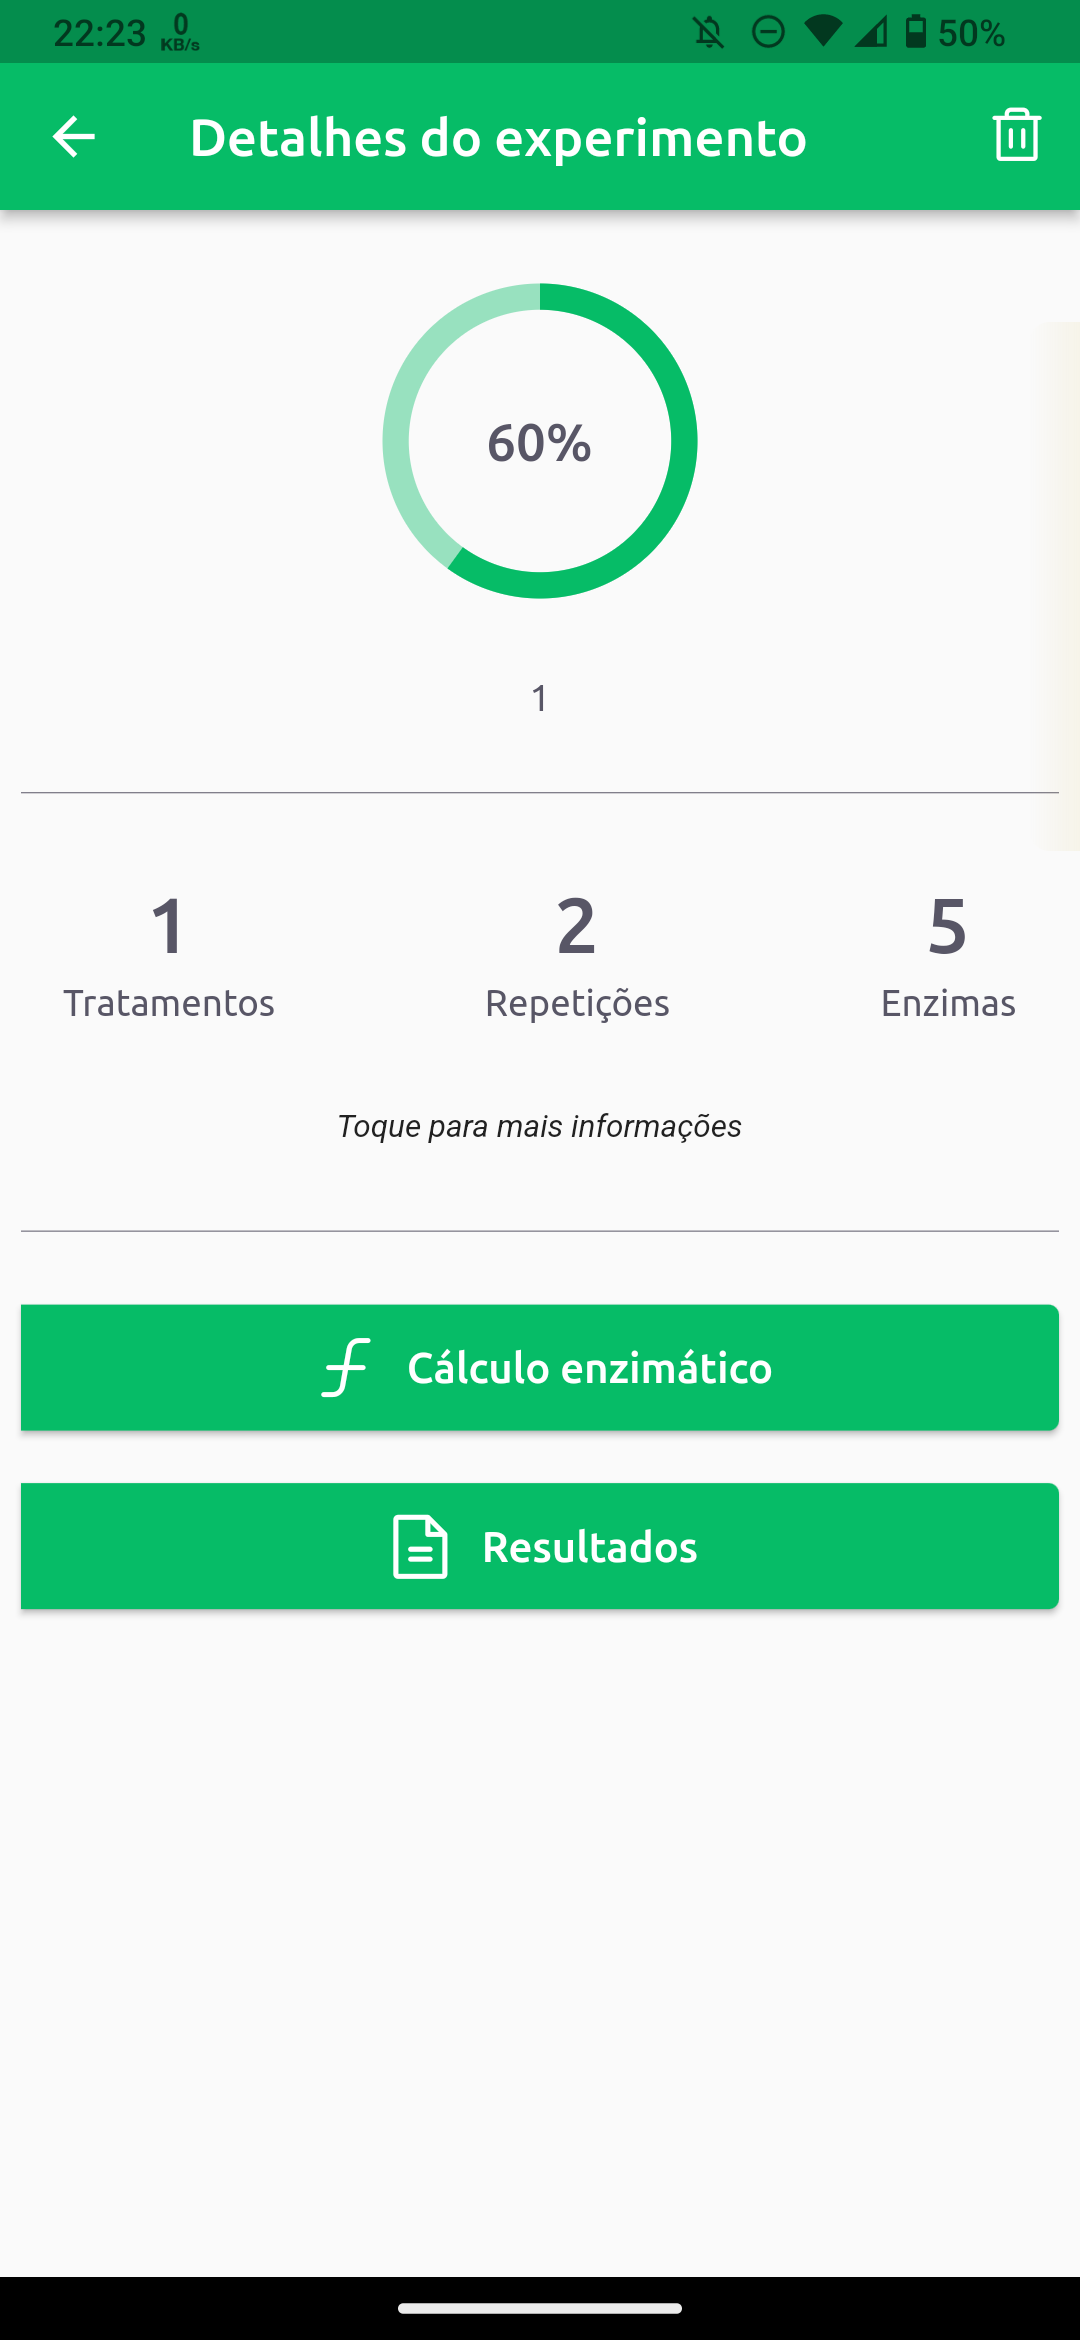
\includegraphics[width=.3\textwidth]{images/enzitech/exp_detalhado3.png}
  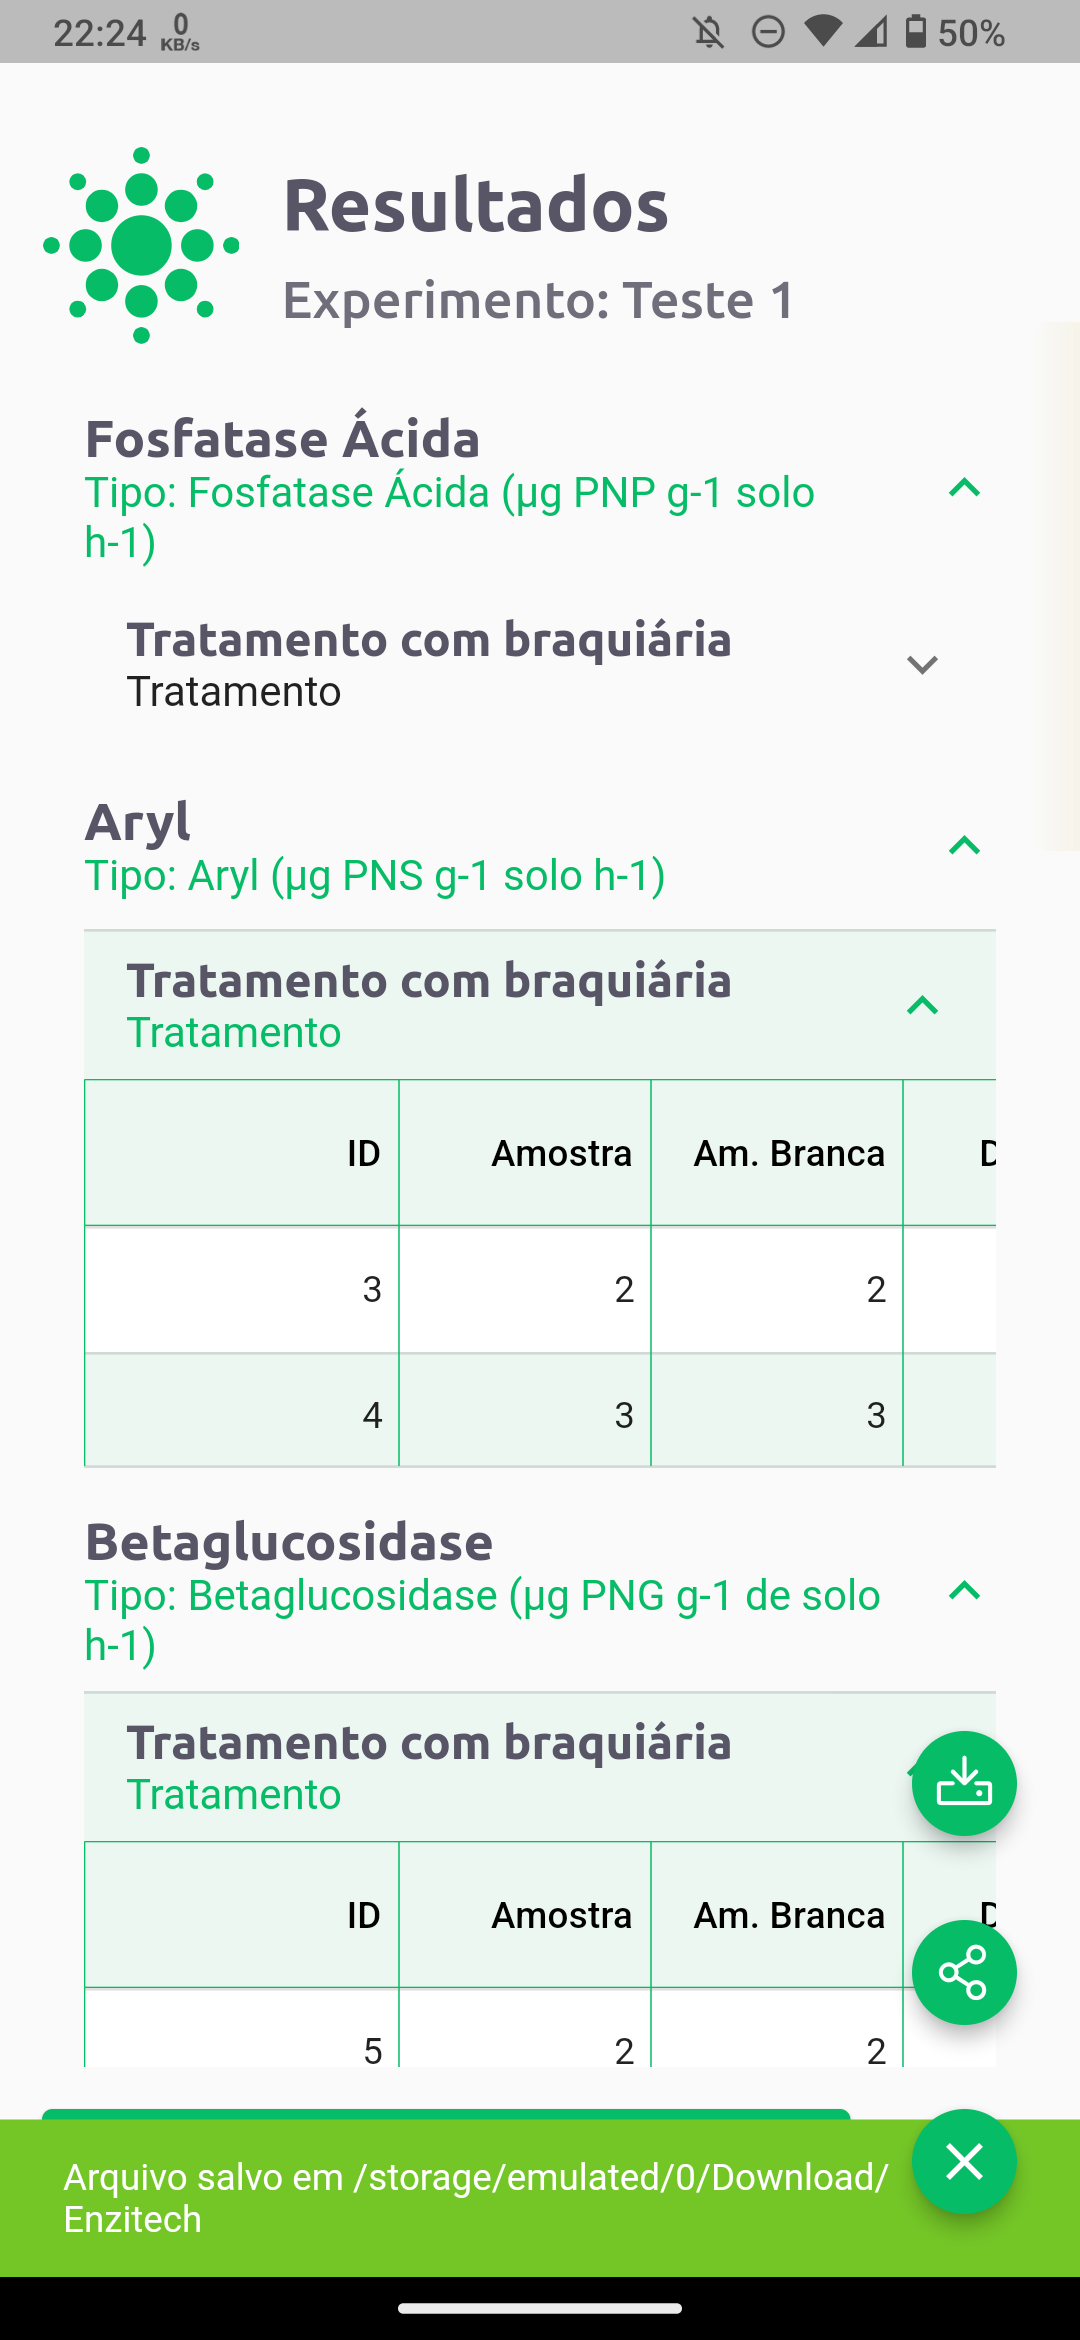
\includegraphics[width=.3\textwidth]{images/enzitech/resultados_salvar.png}

  \vspace{1cm}

  
\includegraphics[width=.3\textwidth]{images/enzitech/resultados_salvar_downloads.png}
  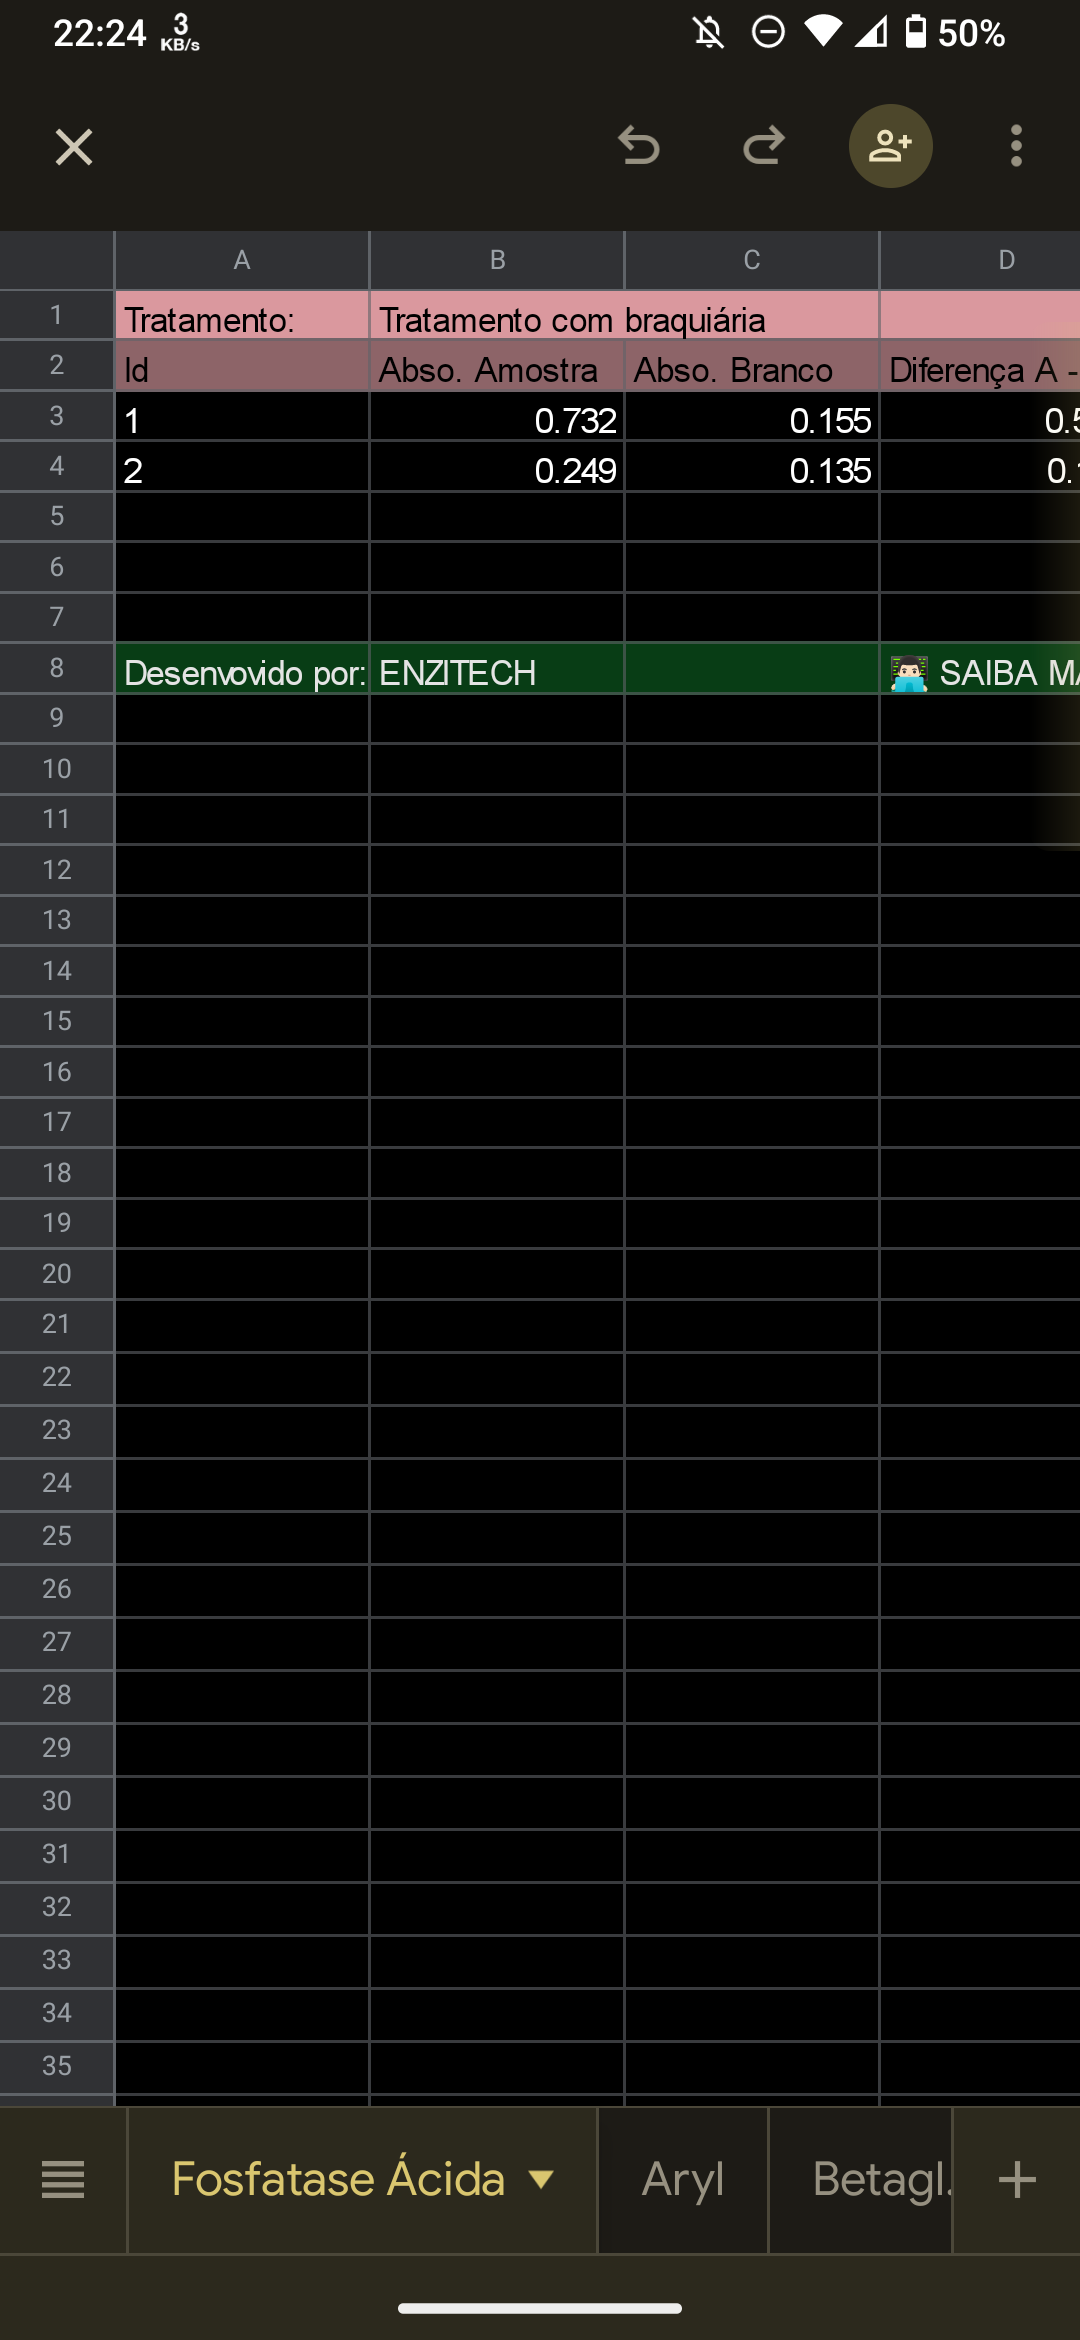
\includegraphics[width=.3\textwidth]{images/enzitech/resultados_salvar_planilha_min.png}
  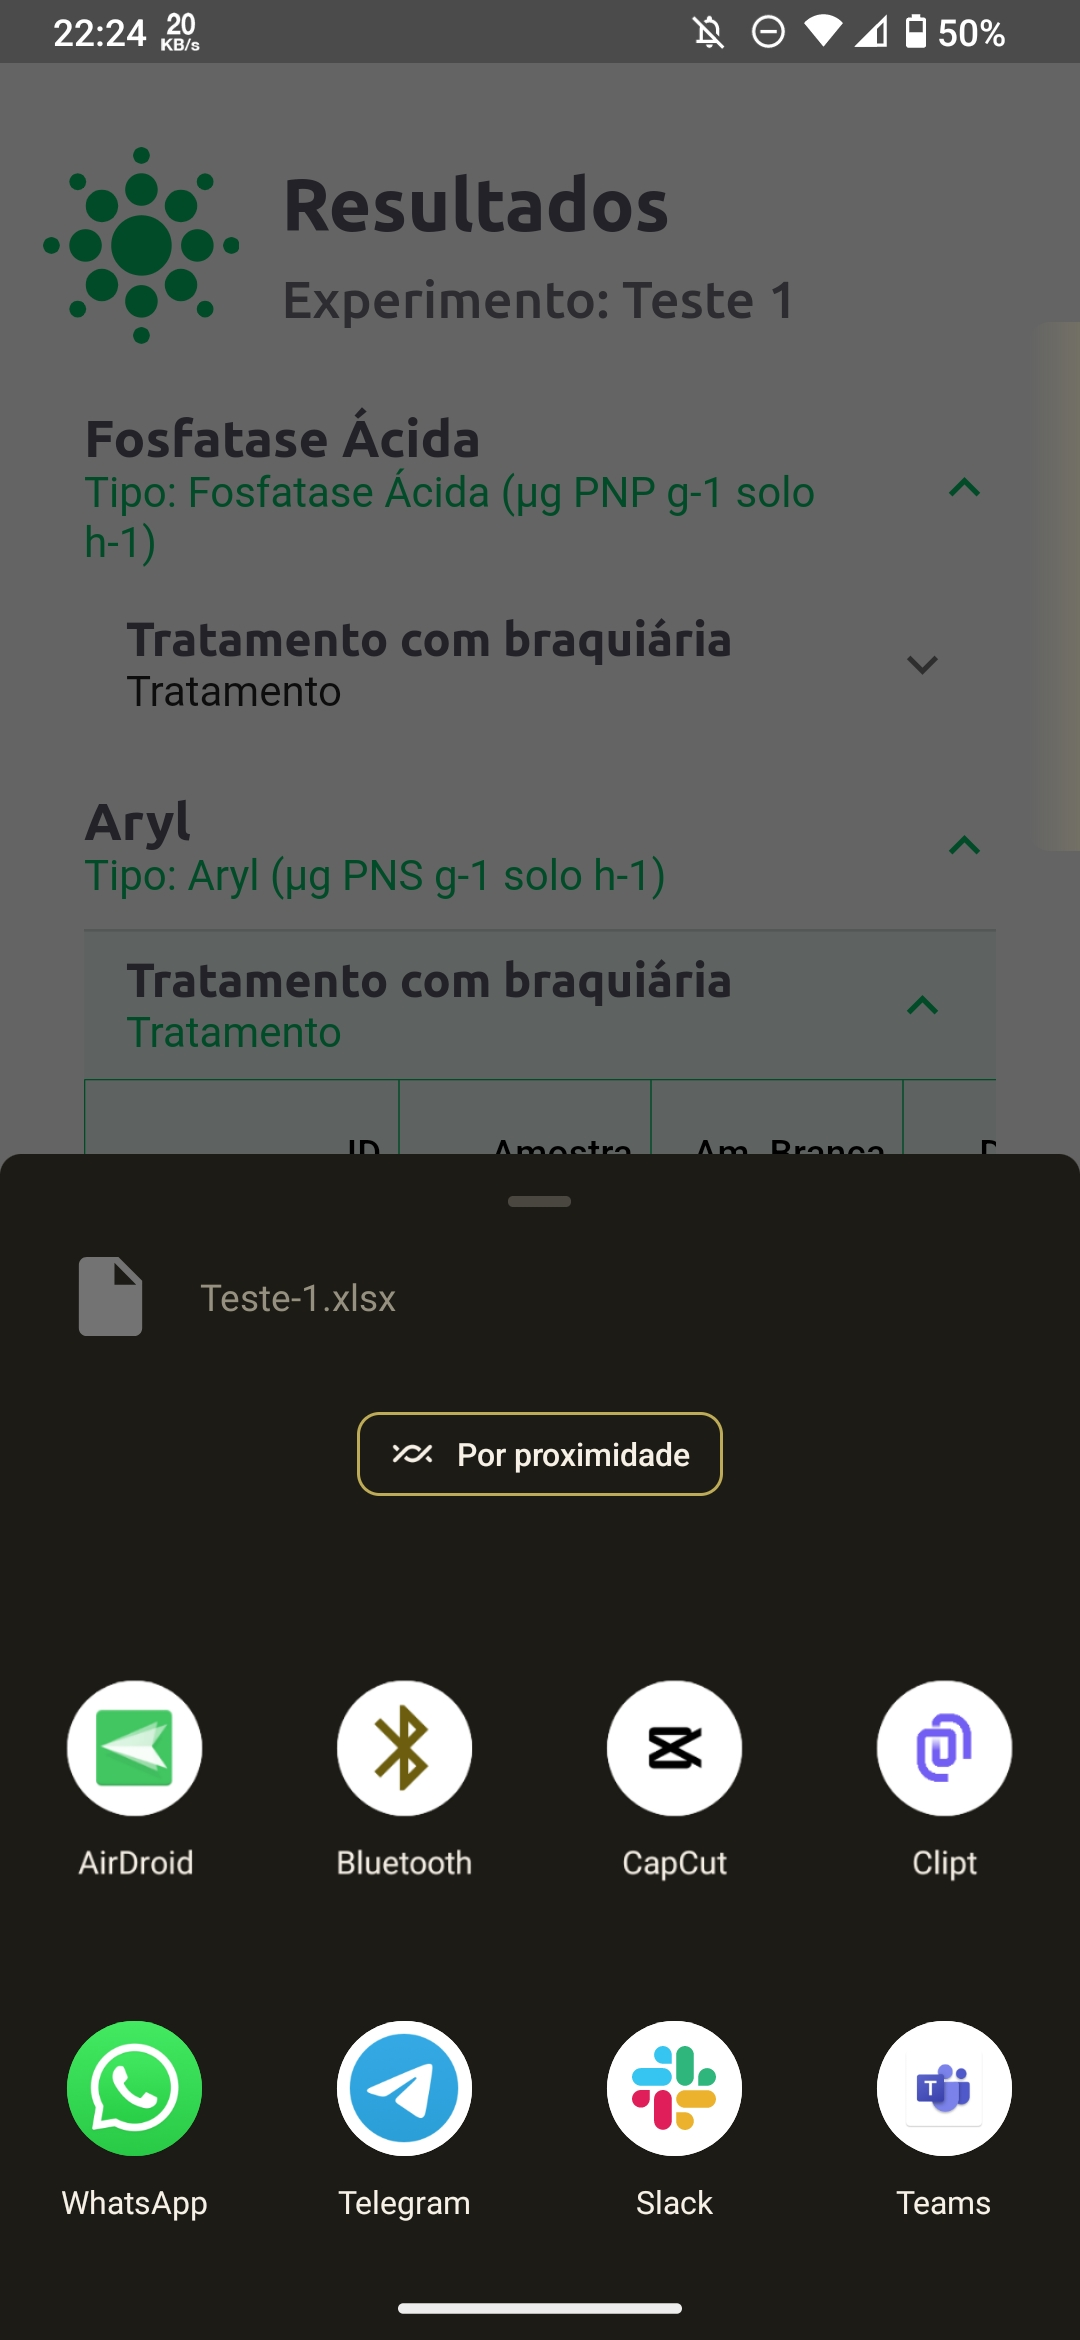
\includegraphics[width=.3\textwidth]{images/enzitech/compartilhar.jpg}

  \caption{Fluxo de visualização e compartilhamento de resultados de um experimento}
  \label{fig:fluxo_resultados}
  \acsfont{Fonte: Aplicativo Enzitech desenvolvido pelo autor}
  
\end{figure}

As duas primeiras imagens do fluxo da \figref{fig:fluxo_resultados} são de experimentos diferentes, a primeira é de um que já foi concluído, nele é possível ver que o usuário tem a ação de cálculo enzimático bloqueado, já na segunda imagem é o experimento que seguirá o fluxo de visualização e compartilhamento dos resultados aqui, este experimento possui um tratamento, duas repetições, e cinco enzimas cadastradas.

Ao entrar nos resultados do experimento, o usuário consegue visualizar de forma organizada todos os dados preenchidos como uma listagem com tabelas para cada combinação de enzima e tratamento feita, nesta tela, é possível salvar o resultado em uma planilha Excel no formato \textsc{nome-do-experimento.xlsx} no armazenamento do dispositivo, como é possível ver na terceira, quarta e quinta imagem do fluxo da \figref{fig:fluxo_resultados}, a planilha é montada seguindo o mesmo padrão, para cada enzima é criado uma página, e dentro de cada página os resultados são montados com suas repetições para cada tratamento do experimento (caso de uso UC10).

Além disso, o usuário pode compartilhar diretamente o arquivo para qualquer \ac{app} externo que suporte esta ação, ao compartilhar um experimento, o salvamento dele também é realizado (caso de uso UC11).

Por fim, o usuário tem acesso à uma tela de configurações na \textit{home} do \ac{app} (\figref{fig:configuracoes_app}), nela é possível ter acesso às seguintes funcionalidades adicionais: informações do \ac{app}, seus dados de login, uma configuração para a ativação e desativação do \textit{AlertDialog} para confirmação da exclusão de itens no \ac{app}, informação da quantidade de resultados de experimentos salvos localmente, informações sobre ambiente e versão do \ac{app} e a opção de deslogar do sistema. Além, disso, como mostrado na última imagem, o \ac{app} tem uma funcionalidade que informa quando o aplicativo fica sem acesso ao servidor, seja por falha no servidor ou por problemas de conexão com a internet. Por fim, o \ac{app} também contempla a funcionalidade de armazenar e consumir dados em \textit{cache} quando não há conexão com a internet disponível, tornando possível a visualização de algumas informações resumidas.

\begin{figure}[H]
\centering
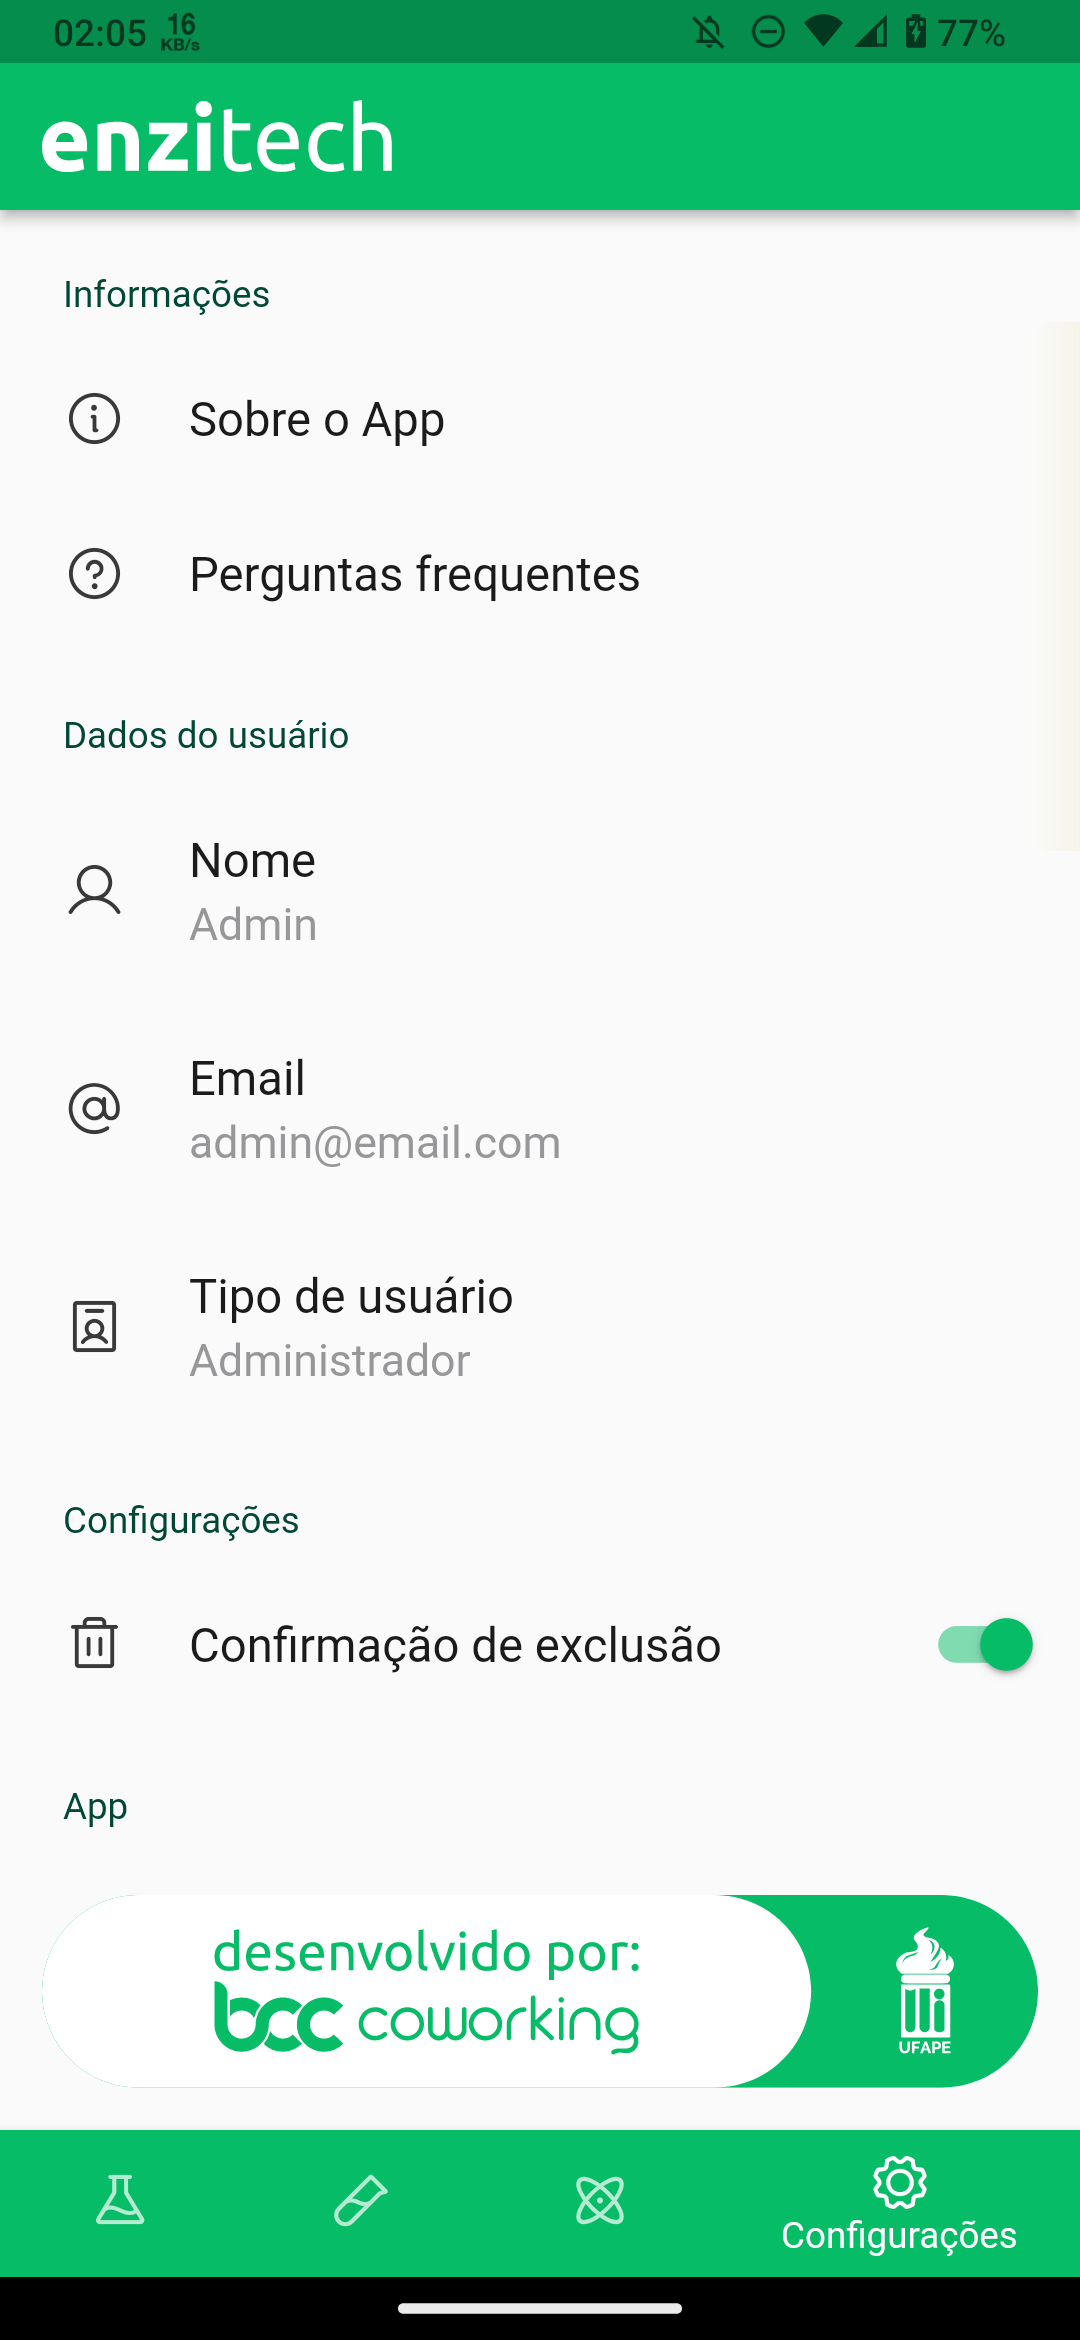
\includegraphics[width=.3\textwidth]{images/enzitech/config.png}\hfill
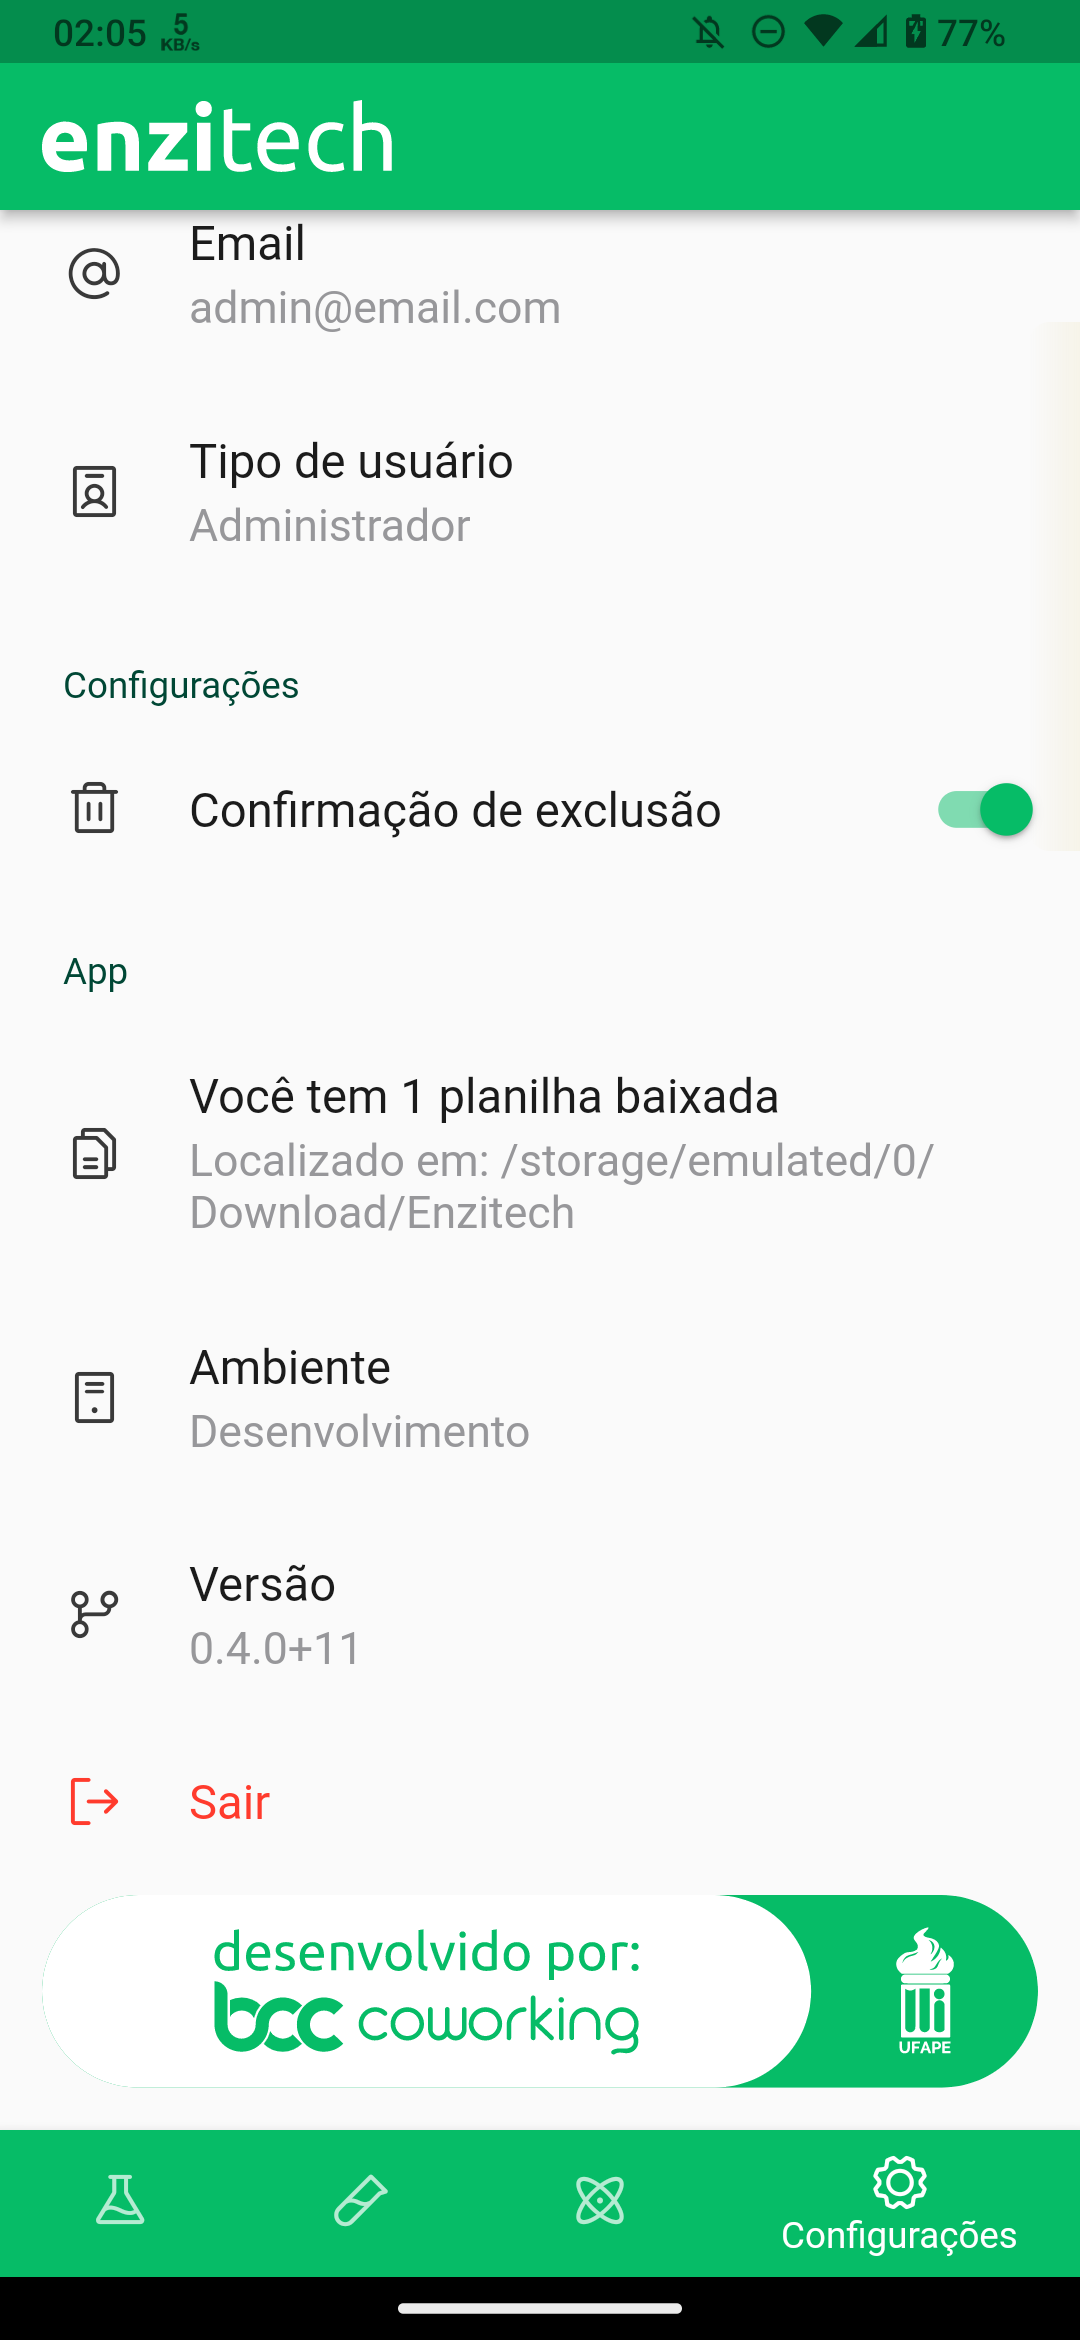
\includegraphics[width=.3\textwidth]{images/enzitech/config2.png}\hfill
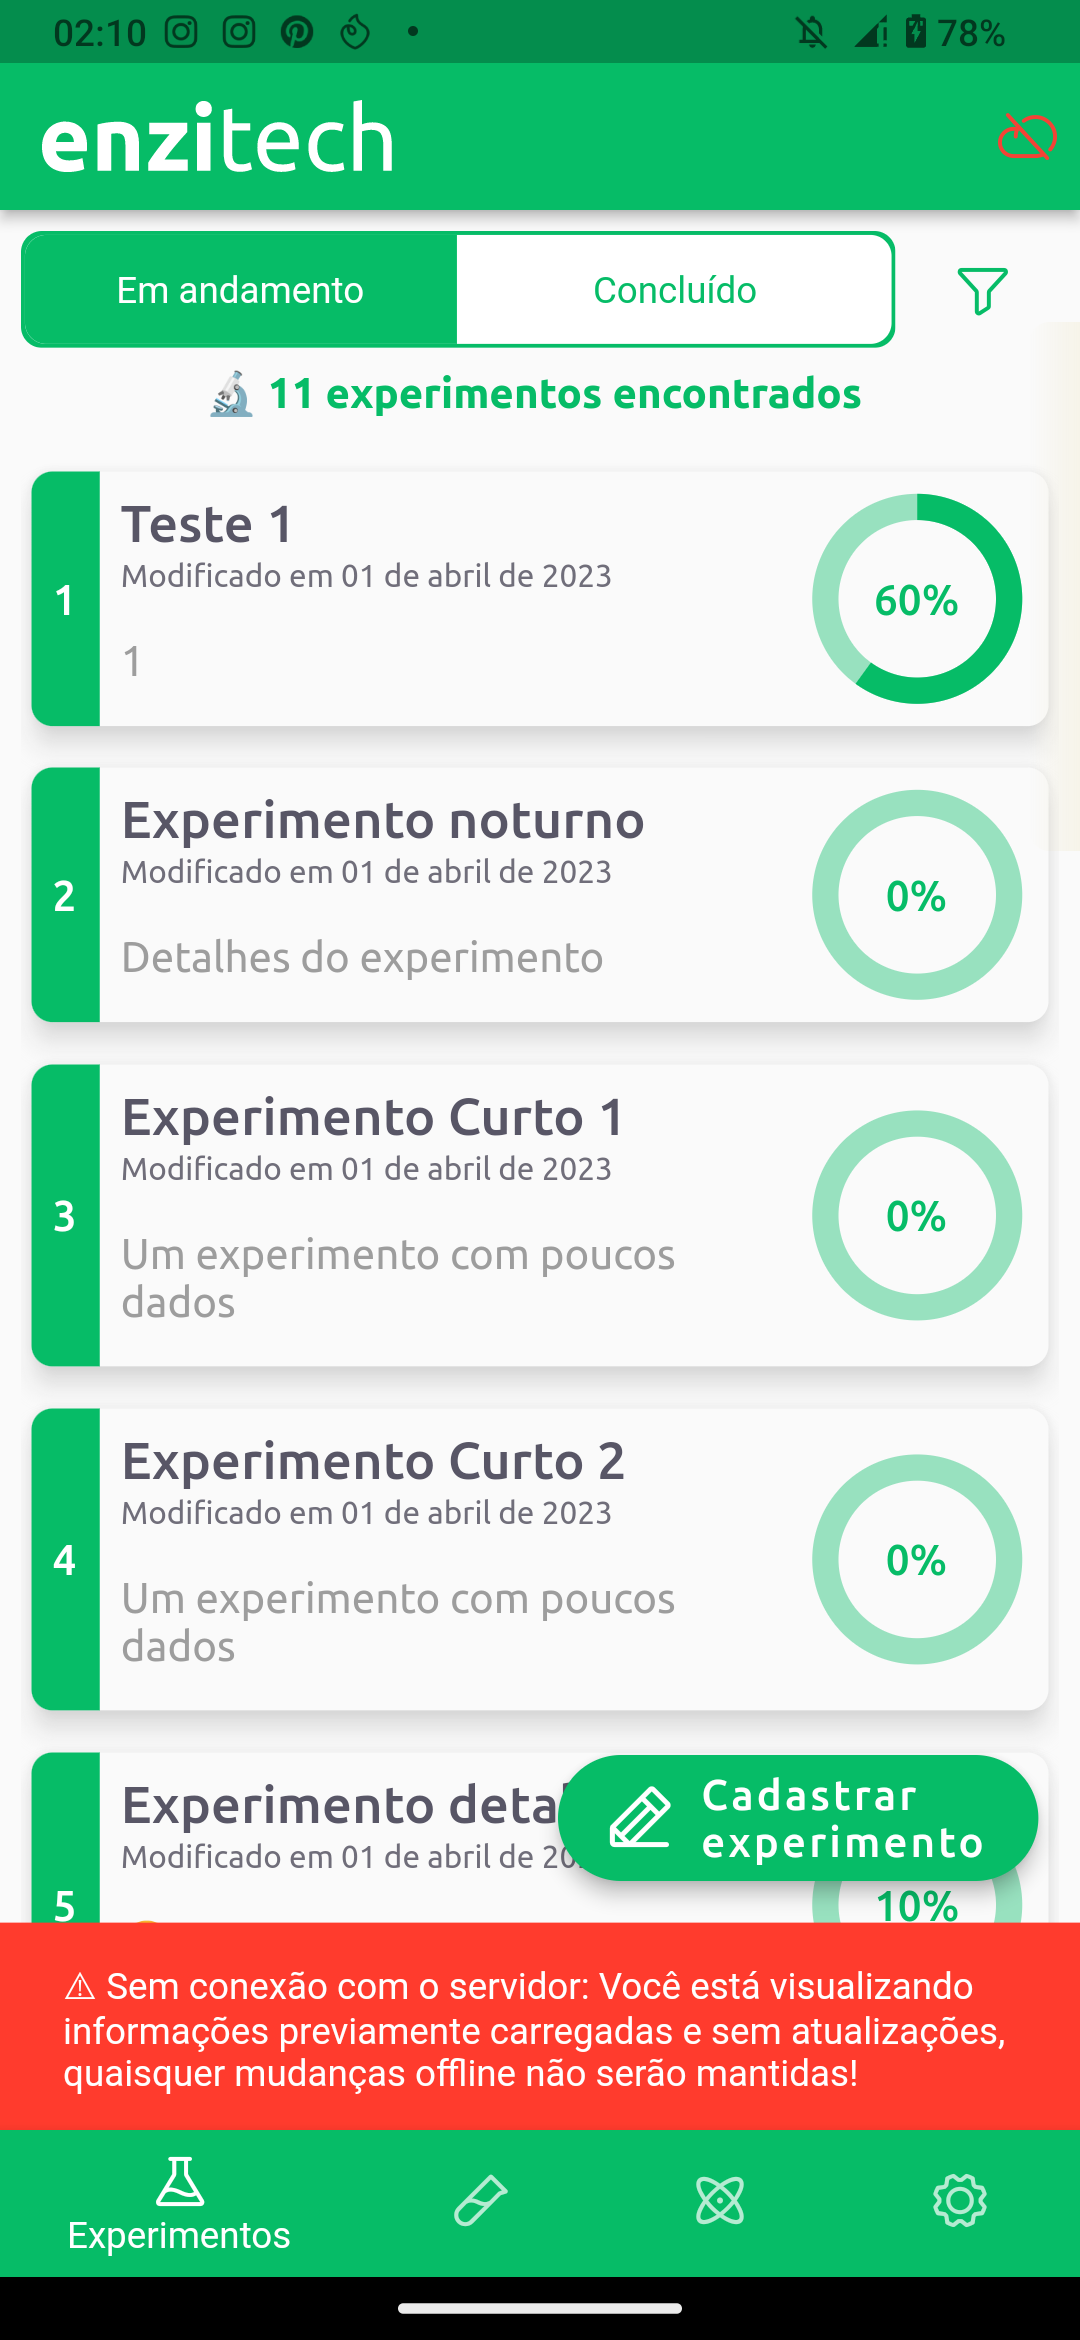
\includegraphics[width=.3\textwidth]{images/enzitech/offline.png}\hfill
\caption{Tela de configurações do \ac{app} do Enzitech}
  \acsfont{Fonte: Aplicativo Enzitech desenvolvido pelo autor}
\label{fig:configuracoes_app}
\end{figure}
